% CVPR 2025 Paper Template; see https://github.com/cvpr-org/author-kit

\documentclass[10pt,twocolumn,letterpaper]{article}
\usepackage{cvpr}           

%
% --- inline annotations
%
\newcommand{\red}[1]{{\color{red}#1}}
\newcommand{\todo}[1]{{\color{red}#1}}
\newcommand{\TODO}[1]{\textbf{\color{red}[TODO: #1]}}
% --- disable by uncommenting  
% \renewcommand{\TODO}[1]{}
% \renewcommand{\todo}[1]{#1}



% It is strongly recommended to use hyperref, especially for the review version.
% hyperref with option pagebackref eases the reviewers' job.
\definecolor{cvprblue}{rgb}{0.21,0.49,0.74}
\usepackage[pagebackref,breaklinks,colorlinks,allcolors=cvprblue]{hyperref}

\def\paperID{12345678}
\def\confName{CVPR}
\def\confYear{2025}

%%%%%%%%% TITLE - PLEASE UPDATE
\title{Frozen Core, Plug-in Precision: Extending a General Multi-Task Edge Perception Model\\without Regression, Validated in a Closed Drone-Racing Loop}

\author{Ambitious AI Researcher\\
AI Research Institute\\
123 AI Avenue, ML City\\
{\tt\small researcher@institute.ai}
}

\begin{document}
\maketitle

\begin{abstract}
%%%%%%%%% ABSTRACT %%%%%%%%%
Small robots benefit from a single onboard multi-task perception model. When one application needs much higher precision on one task, the usual remedies are a separate task-specific network, which adds a second backbone pass, or fine-tuning of the shared model, which risks the other tasks. A demanding example is sub-pixel gate corners for an EKF state estimator in drone racing. We ask whether \emph{read-only} extension suffices: the general model stays completely frozen, and small application-trained modules only read its intermediate features, so the released model and its validated metrics are untouched. Our core is an $\sim$8M-parameter FastViT-SA24 hybrid student with segmentation, inverse-depth, lane and gate-corner heads. We add three heads on its frozen stride-8 features (CornerRefiner, CornerPeakHead, NearGateHead) and two parameter-free steps: global duplicate suppression and a minimum-size filter. Settings are selected in the closed loop of the application. We swap only the detector of a third-party racing stack in Isaac Lab \emph{simulation}. Over 128 flights on final-test seeds that were never examined during development, our system succeeds in 87.5\% of flights versus 82.0\% for the stack's dedicated GateNet detector. The difference is consistent across two independent tests but not significant (sign test $p\approx0.14$), so we claim parity. The general metrics stay identical, \eg TuSimple IoU 0.803 and SUN RGB-D mIoU 0.749. The reparameterized core runs in 26.4\,ms (15\,W) and 14.6\,ms (MAXN) on a Jetson Orin NX. In our study, in-loop pixel precision and duplicate detections explained closed-loop outcomes better than offline crop metrics.
%%%%%%%%% ABSTRACT %%%%%%%%%
\end{abstract}

\section{Introduction}
\label{sec:intro}
%%%%%%%%% INTRODUCTION %%%%%%%%%
Small autonomous robots such as drones and ground vehicles must perceive their surroundings with an onboard computer of a few watts. They are increasingly built around a \emph{single} multi-task perception model. One shared network that predicts semantic segmentation, inverse depth, lanes and object keypoints is attractive on an edge device such as the NVIDIA Jetson Orin NX. It needs one set of weights in memory and one backbone pass per frame. It also offers one energy budget and one artifact to validate, update and maintain. Training such a model on many real and synthetic datasets, and distilling it into a compact student, yields a general perception core that serves many applications at once.

This promise breaks when one application needs much higher precision on a single task than a general model provides. Autonomous drone racing is a demanding example. Vision-based racing systems detect gate corners and fuse them in a filter-based state estimator to correct drift and localize relative to the track~\cite{Foehn2020AlphapilotAutonomous}. Learned racing policies push quadrotors to their physical limits~\cite{Song2023ReachingLimit}. At such speeds, the estimator tolerates only one to two pixels of corner error. Practitioners usually respond in one of two ways. The first is to deploy a separate task-specific network, which adds a second backbone pass to the onboard budget. The second is to fine-tune the shared model on the target task, which risks catastrophic forgetting of the other tasks~\cite{Kirkpatrick2016OvercomingCatastrophic,Wang2023ComprehensiveSurvey}. Multi-task learning has a related problem: re-weighting losses toward one task trades accuracy on the others and does not reliably improve the target task~\cite{Xin2022DoCurrent,Lin2023DualbalancingMultitask}.

A third option is well known as a mechanism: keep the trunk frozen and attach new heads that read its features, as in probing, multi-head frozen trunks and side networks. That non-regression follows from this design is a simple identity, not a technical contribution. What is less clear is whether read-only extension is \emph{enough} when the target task is precision-critical and the downstream consumer is a closed-loop estimator, not an offline benchmark. A frozen, general-purpose representation may simply not contain the precision needed. Parameter-efficient methods such as prompts and adapters~\cite{Jia2022VisualPrompt,Chen2022AdaptformerAdapting,Chen2022VisionTransformer} and weight-space interpolation~\cite{Wortsman2021RobustFinetuning} make a different trade-off. They deliberately adapt the shared representation to gain accuracy, at the price of a modified forward pass or a new weight set that must be re-validated. Our question is the opposite one: how far can an application get while leaving a released, validated core exactly as it is?

We study this question for one application in simulation. The core is an $\sim$8M-parameter hybrid FastViT-SA24 student with heads for segmentation, inverse depth, lanes and dense gate corners. When reparameterized, it runs at 26.4\,ms per frame on a Jetson Orin NX in 15\,W mode. The application is a third-party drone racing stack in Isaac Lab, made of a learned racing policy and an EKF state estimator. The stack comes with its own simulator-trained gate detector, GateNet, which serves as our baseline. We swap only the detector; the policy, estimator and camera pipeline stay unchanged.

With the core's gate head alone, the system reached 37.5\% success against 78.1\% for GateNet. Attempts to obtain precision inside the core gave no closed-loop gain within loop noise: fine-tuning on simulator renders, higher corner loss weights, a stride-2 corner head and model soups. Their cost on general metrics also grew with the corner weight. In-loop diagnosis showed that the gap came from pixel precision rather than recall. We closed it with three application-trained heads on frozen stride-8 features. A \emph{CornerRefiner} performs second-pass sub-pixel refinement. A \emph{CornerPeakHead} confirms weak detections. A \emph{NearGateHead} handles gates that fill the frame. Two parameter-free filters complete the pipeline: global duplicate suppression and a minimum-size filter.

Our contributions are:
\begin{itemize}
    \item An empirical answer to the sufficiency question for one precision-critical application. Read-only heads on the frozen features of a general edge model reach closed-loop parity with a dedicated, application-trained detector. On two independent sets of final-test seeds (128 flights per arm), our system completes 87.5\% of flights versus 82.0\% for GateNet. The difference is consistent but not significant ($p\approx0.14$). The released core, and every general metric validated on it, stays unchanged.
    \item Closed-loop diagnostics that locate the bottleneck. These are in-loop corner error binned by gate size, the sensitivity of the EKF to duplicate detections, and estimator error binned by distance. Together they show that pixel precision and duplicate-free outputs, not found rate, determined success in this loop.
    \item A deployment characterization of the core on a Jetson Orin NX. It shows that structural reparameterization is what makes the shared core fit the 30\,Hz camera rate at 15\,W (44.2$\to$26.4\,ms).
\end{itemize}
All closed-loop results are in simulation. We study one application against one dedicated baseline.
%%%%%%%%% INTRODUCTION %%%%%%%%%

\section{Related Work}
\label{sec:related_work}
%%%%%%%%% RELATED WORK %%%%%%%%%
\paragraph{Multi-task and efficient perception backbones.}
A shared encoder with several task heads is a natural fit for resource-constrained robots. It amortizes computation across segmentation, depth, lanes and keypoints. The central difficulty is interference among tasks. Many multi-task optimization methods re-weight losses or manipulate gradients. Dual-balancing~\cite{Lin2023DualbalancingMultitask}, for instance, applies a logarithmic transform to each loss and normalizes gradient magnitudes. A large-scale study found that such optimizers often fail to beat a well-tuned weighted sum of losses~\cite{Xin2022DoCurrent}. This suggests a real trade-off between tasks in a shared model. Our experience is consistent with this view: raising the corner loss weight (10, 40, 100) increased the cost on general metrics without a measurable closed-loop gain.

\paragraph{Heads on frozen features.}
Training new heads on a frozen trunk is standard practice. Examples are linear probing, multi-head networks that share a fixed trunk, and side networks that run next to a frozen backbone and combine its features with their own. Non-interference with the original outputs is a direct property of these designs. We use this mechanism unchanged and do not claim it as new. Our focus is empirical. We ask whether this kind of extension is enough for a task whose precision requirement is set by a closed-loop estimator, and which in-loop factors decide that.

\paragraph{Extending pretrained models by adapting them.}
Fine-tuning a pretrained network overwrites weights that earlier tasks rely on. Elastic weight consolidation slows learning on weights important for old tasks~\cite{Kirkpatrick2016OvercomingCatastrophic}, and continual learning frames the problem as a stability--plasticity trade-off~\cite{Wang2023ComprehensiveSurvey}. WiSE-FT~\cite{Wortsman2021RobustFinetuning} interpolates between pretrained and fine-tuned weights to recover robustness. Parameter-efficient transfer keeps backbone weights fixed but deliberately changes the representation. Visual Prompt Tuning~\cite{Jia2022VisualPrompt} prepends learnable tokens. AdaptFormer~\cite{Chen2022AdaptformerAdapting} inserts parallel modules into the MLP blocks of a ViT. ViT-Adapter~\cite{Chen2022VisionTransformer} injects image priors for dense prediction. These methods aim at higher target accuracy through adaptation and can match full fine-tuning. Their outputs on the original tasks are not guaranteed to be preserved, by design. They target a different point of the trade-off than read-only extension: more plasticity in exchange for re-validating the shared model.

\paragraph{Gate detection and perception-in-the-loop for drone racing.}
AlphaPilot~\cite{Foehn2020AlphapilotAutonomous} couples learned gate detection with nonlinear filtering and exploits multiple simultaneous gate detections to compensate for drift. Song~\etal~\cite{Song2023ReachingLimit} show that reinforcement learning policies can outperform optimal control in racing because they optimize a task-level objective directly. This highlights that closed-loop performance depends on factors that intermediate objectives do not capture. The stack we build on follows this pattern. A learned policy is fed by an EKF that fuses a map prior with gate-corner observations, and the stack ships with a dedicated detector, GateNet, trained on simulator data. We replace only the detector and report closed-loop success.
%%%%%%%%% RELATED WORK %%%%%%%%%

\section{Methodology}
\label{sec:method}
%%%%%%%%% METHOD %%%%%%%%%
\begin{figure*}[t]
  \centering
  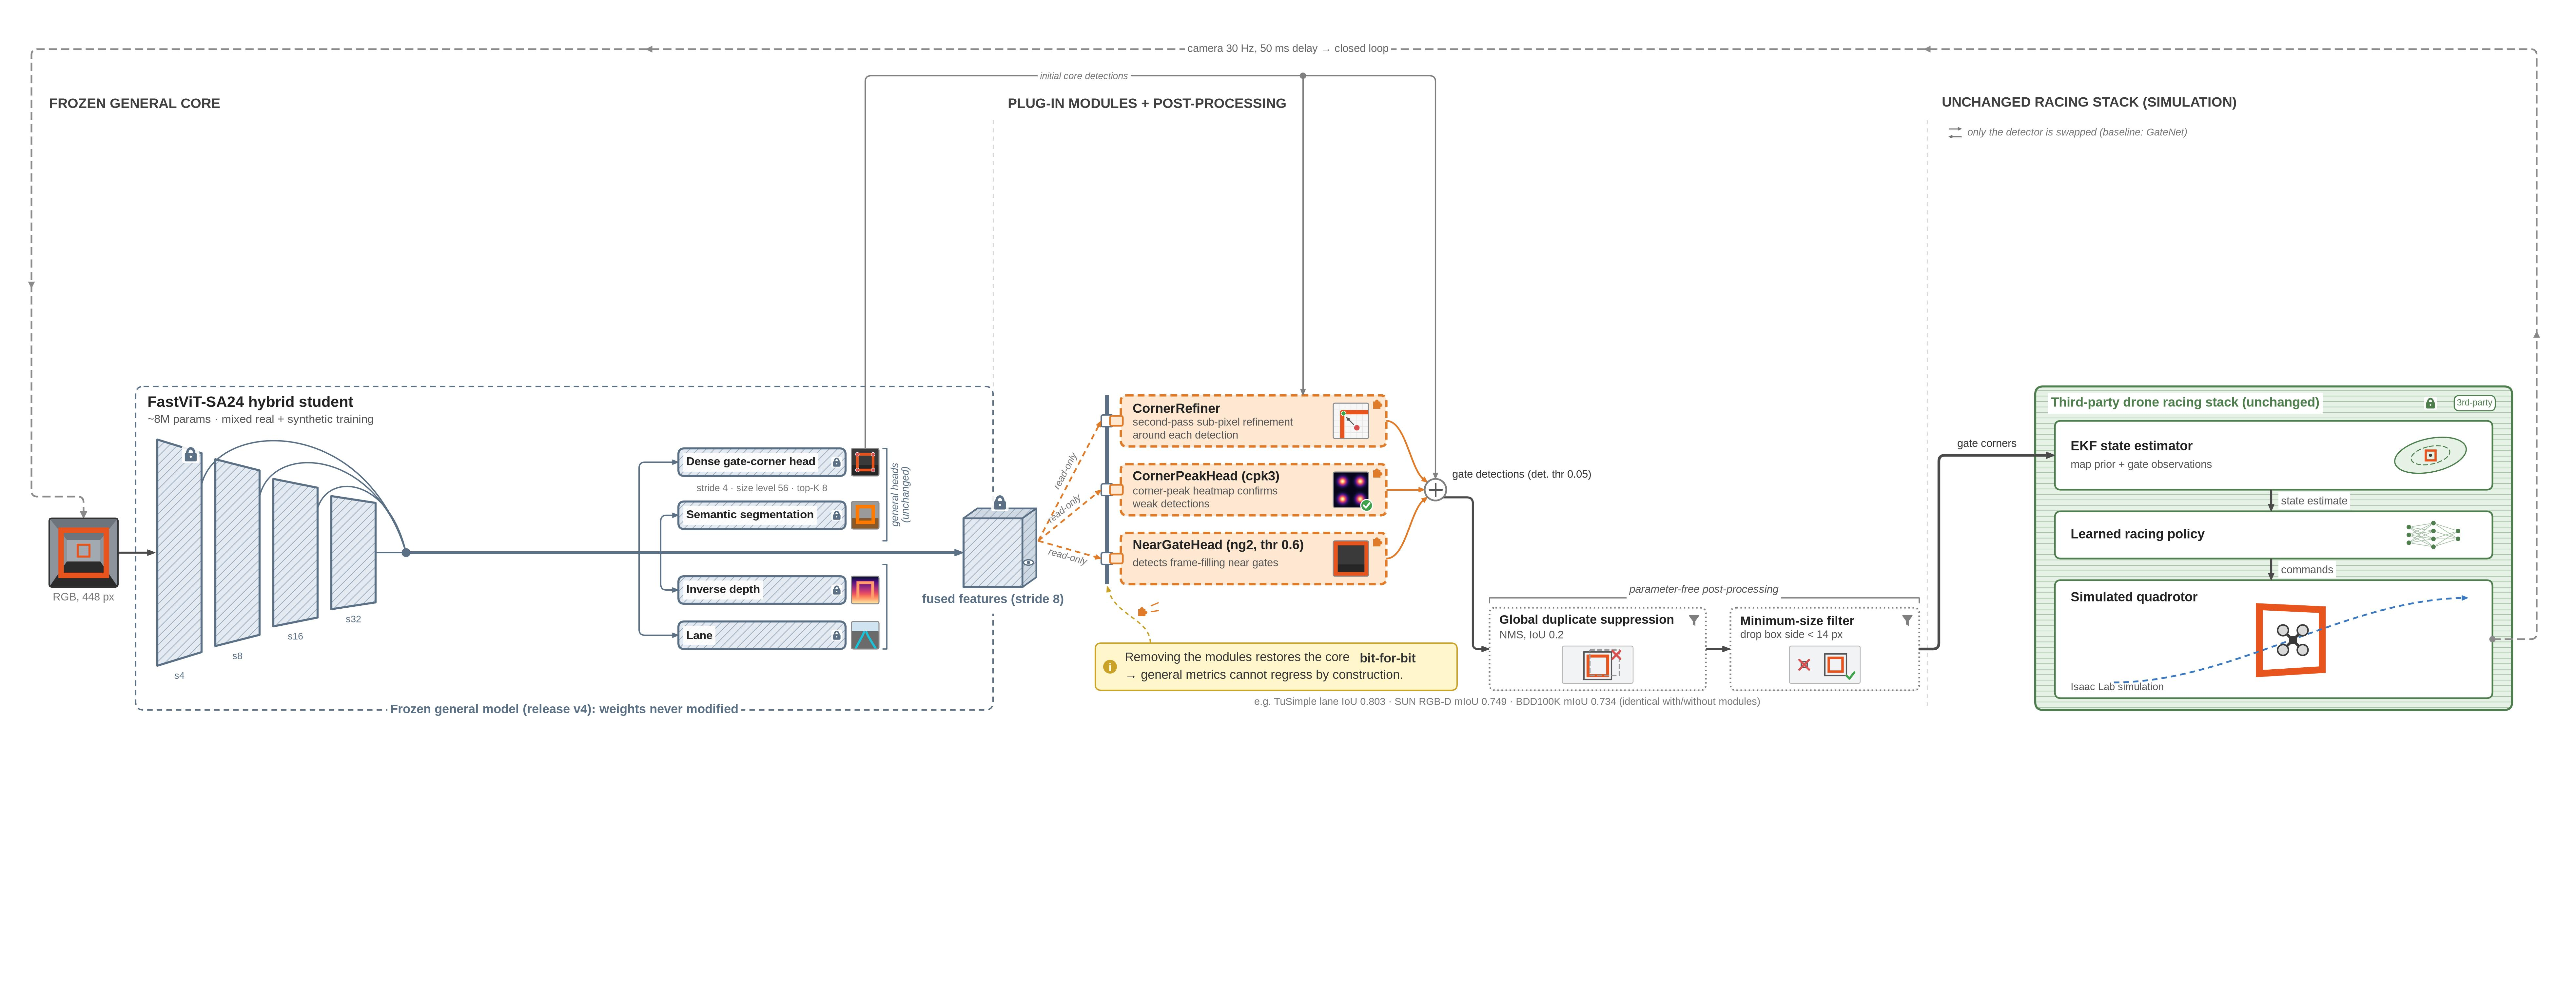
\includegraphics[width=\textwidth]{figures/fig_frozen_core_plugin_module_framework.jpg}
  \caption{Overview of the frozen general model and its plug-in modules. \textbf{Left:} the frozen multi-task student (FastViT-SA24 hybrid, $\sim$8M parameters, trained at 448\,px) runs four general heads: semantic segmentation, inverse depth, lane, and a dense gate-corner head (stride 4, size level 56, top-K 8). Its weights are never modified. \textbf{Center:} three small trainable heads have read-only access to the frozen stride-8 fused features. CornerRefiner refines each detected corner to sub-pixel accuracy in a second pass. CornerPeakHead (cpk3) confirms weak detections with a corner-peak heatmap. NearGateHead (ng2, threshold 0.6) detects near gates that fill the frame. Their outputs are merged with the core's initial detections (detection threshold 0.05). Two steps without learned parameters follow: global duplicate suppression (NMS, IoU 0.2) and a filter that drops boxes with a side under 14\,px. \textbf{Right:} the filtered gate corners feed an unchanged third-party drone racing stack in Isaac Lab simulation, consisting of an EKF state estimator and a learned racing policy. Only the detector is swapped; the baseline is GateNet. Removing the modules leaves the core's outputs unchanged. Hatching marks frozen parts, dashed orange borders mark trainable modules, and dotted borders mark steps without learned parameters.}
  \label{fig:framework}
\end{figure*}

\Cref{fig:framework} gives an overview of the approach. We first formalize frozen-core extension (\cref{sec:formulation}). We then describe the general core (\cref{sec:core}), the plug-in modules for gate corners (\cref{sec:modules}) and the parameter-free post-processing (\cref{sec:postproc}).

\subsection{Problem formulation: frozen-core extension}
\label{sec:formulation}
Let $x$ be an input image and let $f_\theta$ be the general multi-task model with parameters $\theta$. We write $f_\theta$ as a shared encoder--decoder $\phi_\theta$ that produces fused intermediate features, followed by task heads $h_k$:
\begin{equation}
  F = \phi_\theta(x), \qquad y_k = h_k(F), \quad k \in \mathcal{K},
  \label{eq:core}
\end{equation}
where $\mathcal{K} = \{\text{seg}, \text{inv.\ depth}, \text{lane}, \text{gate corner}\}$ and $F$ denotes the stride-8 fused feature map. All parameters $\theta$, including those of the heads, are frozen once the core is released.

A \emph{plug-in module} $g_\psi$ with its own parameters $\psi$ reads $F$, and optionally the core's own detections $y_{\text{gate}}$, and outputs an application-specific prediction
\begin{equation}
  \hat{y}_{\text{app}} = g_\psi\big(\operatorname{sg}(F),\, y_{\text{gate}}\big),
  \label{eq:module}
\end{equation}
where $\operatorname{sg}(\cdot)$ is a stop-gradient. During training only $\psi$ is updated, by minimizing an application loss $\mathcal{L}_{\text{app}}(\hat{y}_{\text{app}}, y^\star)$ against application targets $y^\star$. Because $g_\psi$ never writes into $\phi_\theta$ or any $h_k$, the general outputs satisfy
\begin{equation}
  h_k\big(\phi_\theta(x)\big)\big|_{\text{with } g_\psi} \equiv h_k\big(\phi_\theta(x)\big)\big|_{\text{without } g_\psi}, \quad \forall x,\ \forall k \in \mathcal{K}.
  \label{eq:nonregression}
\end{equation}
\Cref{eq:nonregression} is a simple identity of computation, shared by any frozen-trunk design. We state it because of its operational consequence, not because it is new. The released core, its export and the benchmark results validated on it remain valid however many modules are added, and several modules $g_{\psi_1},\dots,g_{\psi_M}$ can be attached in parallel without interacting through the core.

\paragraph{Closed-loop selection.}
For our application the quantity of interest is the success rate of the full robot system, not an offline score. Let $c$ be a configuration (a set of modules plus post-processing settings), and let $S(c; \mathcal{D})$ be the fraction of successful flights over a seed set $\mathcal{D}$. We choose
\begin{equation}
  c^\star = \arg\max_{c \in \mathcal{C}} S(c; \mathcal{D}_{\text{val}}),
  \label{eq:selection}
\end{equation}
and report $S(c^\star; \mathcal{D}_{\text{test}})$ on disjoint final-test seeds $\mathcal{D}_{\text{test}}$ (\cref{sec:setup}). Offline metrics serve only as diagnostics.

\subsection{General multi-task core}
\label{sec:core}
The core is a multi-task student built on a FastViT-SA24 hybrid backbone with $\sim$8M parameters, trained at a 448\,px input resolution. It is trained and distilled on mixed real and synthetic data. The data cover segmentation sets from city, indoor, off-road and aerial domains, TuSimple lanes, and real and simulated racing gates. The core has four heads: semantic segmentation, inverse depth, lanes, and a dense gate-corner head that operates at stride 4 with a single size level of 56 and returns the top-$K{=}8$ gate candidates per frame. We refer to this model as \emph{release v4}. It is frozen for all experiments, and the general metrics (\cref{sec:general}) refer to this release at its 448\,px training resolution.

\paragraph{Resolutions and numerical identity.}
In the racing loop the camera pipeline supplies an adaptive 384$\times$384 crop, so the deployed core and all Orin timings (\cref{sec:edge}) use 384$\times$384 inputs. For deployment the hybrid backbone is structurally reparameterized and exported with TensorRT fp16. \Cref{eq:nonregression} holds exactly for a fixed execution backend and engine. If the core and modules were compiled into a single fused engine, the kernel choices of the builder could change fp16 rounding. The safe deployment pattern is therefore to keep the core as its own engine that additionally exposes $F$, with the modules consuming $F$ in a separate engine.

\subsection{Plug-in modules for sub-pixel gate corners}
\label{sec:modules}
The closed-loop diagnosis (\cref{sec:ablation}) showed that the frozen core finds gates but localizes their corners too coarsely for the EKF. The median in-loop corner error was 3.5\,px versus 0.97\,px for GateNet, and the error grew with apparent gate size. We address this with heads that all read the frozen stride-8 fused features $F$ (\cref{fig:framework}, center).

\paragraph{Synthesised single-corner peaks (step B).}
As a first, purely output-side step, we derive single-corner peaks from the core's own dense corner predictions. This lets the pipeline emit a corner even when only part of a gate's evidence is strong. The step has no trainable parameters and does not touch $\theta$.

\paragraph{CornerRefiner.}
Given the initial corner locations from the core's dense head, the CornerRefiner reads $F$ in the neighborhood of each corner and predicts a sub-pixel correction. It thus turns the coarse stride-4 output into the sub-pixel measurements the estimator expects.

\paragraph{CornerPeakHead (cpk3).}
The CornerPeakHead predicts a corner-peak heatmap from $F$. Its role is confirmation: a weak core detection is kept only if corner peaks support it. This allows a low detection threshold of 0.05 for the core's gate head, which recovers low-confidence gates without admitting unsupported candidates.

\paragraph{NearGateHead (ng2).}
Corner error is largest for gates that fill the frame. Gates larger than 250\,px had a 26\,px median error for the core at step B, compared with 9.4\,px for GateNet. The NearGateHead is a dedicated detection head for such gates. It operates on $F$ with a confidence threshold of 0.6, and its detections are merged with those of the core.

\paragraph{Module interface and training.}
All three modules are trainable heads trained for the gate application under \cref{eq:module}. They take $F$ (and, for CornerRefiner and CornerPeakHead, the core's gate candidates) as input and are optimized against gate-corner targets with gradients stopped at $F$. The modules are therefore application-specific, just like GateNet. In particular, the NearGateHead is itself a small dedicated detector. The difference from deploying GateNet is not general versus dedicated output. It is that all application-specific computation runs as heads on features the core already computes, so there is no second backbone pass and no second image pipeline. We combine the core detections, filtered by CornerPeakHead and refined by CornerRefiner, with the NearGateHead detections, and call this configuration \emph{val\_H}. None of the modules changes $\theta$, so \cref{eq:nonregression} holds for any subset of them.

\subsection{Parameter-free post-processing}
\label{sec:postproc}
\paragraph{Global duplicate suppression.}
Detections now come from three sources: the core head, the confirmed weak detections and the NearGateHead. One gate can therefore be reported more than once. For the EKF, two observations of the same gate are a severe failure: adding small near-gate detections without deduplication collapsed success to 15.6\%. We apply non-maximum suppression jointly across all sources. For gate boxes $B_i, B_j$ (the bounding boxes of the four corners) we use
\begin{equation}
  \operatorname{IoU}(B_i, B_j) = \frac{|B_i \cap B_j|}{|B_i \cup B_j|},
  \label{eq:iou}
\end{equation}
and, visiting detections in order of decreasing confidence, discard $B_j$ if $\operatorname{IoU}(B_i, B_j) > \tau$ for any kept $B_i$, with $\tau = 0.2$. The low threshold reflects that gates on a racing track rarely overlap strongly in the image, whereas duplicates of one gate do. We call this configuration \emph{val\_DS}.

\paragraph{Minimum-size filter.}
Very small boxes yield unreliable corners and are easily confused with decoys. We keep a detection only if
\begin{equation}
  \min(w_j, h_j) \geq s_{\min}, \qquad s_{\min} = 14\ \text{px},
  \label{eq:minsize}
\end{equation}
where $w_j, h_j$ are the box width and height. We chose $s_{\min}$ on validation seeds (\emph{min14}, \cref{sec:ablation}).
%%%%%%%%% METHOD %%%%%%%%%

\section{Experiments}
\label{sec:experiments}
%%%%%%%%% EXPERIMENTS %%%%%%%%%
\subsection{Experimental setup and closed-loop protocol}
\label{sec:setup}
\begin{figure*}[t]
  \centering
  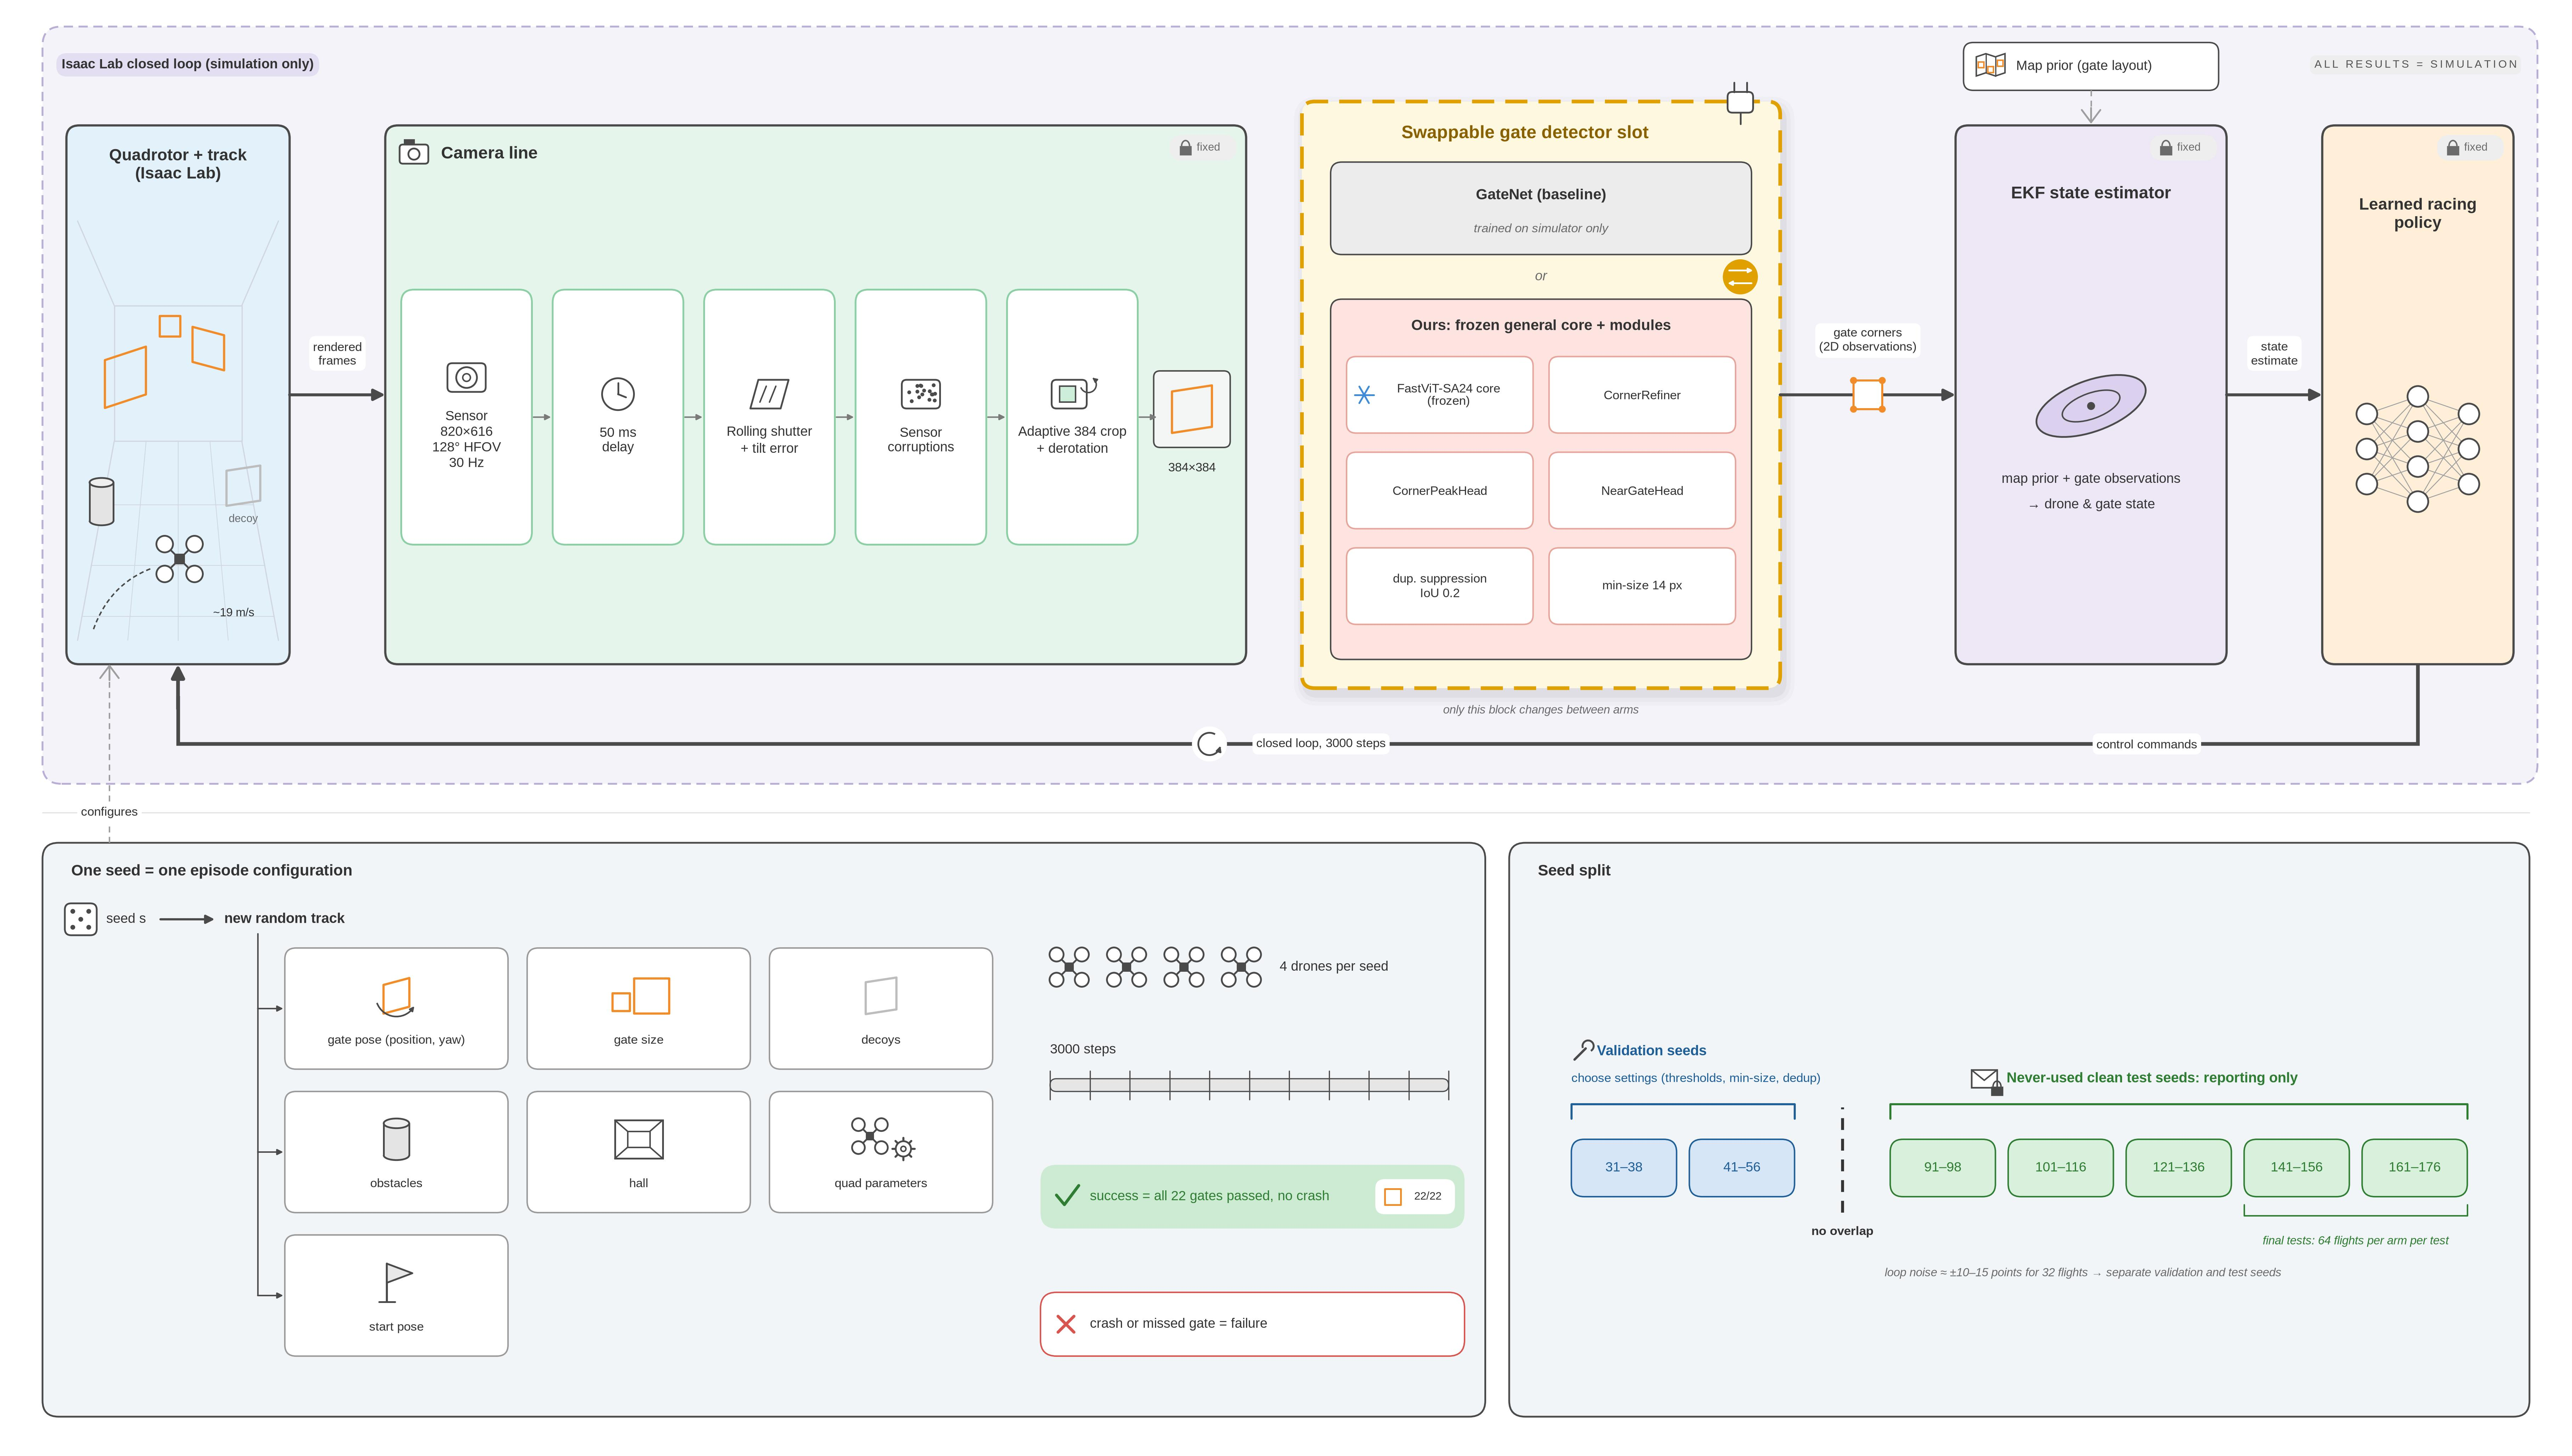
\includegraphics[width=\textwidth]{figures/fig_closed_loop_evaluation_pipeline.jpg}
  \caption{Closed-loop evaluation protocol in Isaac Lab simulation (no real-flight results). \textbf{Top:} rendered frames pass through a fixed camera line (820$\times$616 sensor, 128$^\circ$ HFOV, 30\,Hz, 50\,ms delay, rolling shutter with tilt error, sensor corruptions, and an adaptive 384$\times$384 crop with derotation). A swappable gate detector then outputs 2D gate-corner observations. The detector is either the simulator-trained GateNet baseline or our frozen FastViT-SA24 core with CornerRefiner, CornerPeakHead, NearGateHead, duplicate suppression (IoU 0.2) and a 14\,px minimum-size filter. An EKF fuses these observations with a map prior of the gate layout, and a learned racing policy sends control commands back to the quadrotor. Only the detector changes between arms. \textbf{Bottom left:} each seed generates a new random track with its own gate poses and sizes, decoys, obstacles, hall, quadrotor parameters and start pose. Four drones fly each seed for 3000 steps, and a flight succeeds only if all 22 gates are passed without a crash. \textbf{Bottom right:} because loop noise is about $\pm$10--15 points for 32 flights, settings are chosen on validation seeds (31--38, 41--56). The final tests (141--156, 161--176, never examined before the configuration was frozen) use 64 flights per arm each.}
  \label{fig:pipeline}
\end{figure*}

\paragraph{Racing stack.}
We use a third-party drone racing stack in Isaac Lab (\cref{fig:pipeline}). It consists of a fixed learned racing policy and an EKF state estimator that fuses a map prior of the gate layout with 2D gate-corner observations. The camera line is also fixed: an 820$\times$616 sensor with 128$^\circ$ HFOV at 30\,Hz, 50\,ms delay, rolling shutter, tilt error, sensor corruptions, and an adaptive 384-pixel crop with derotation. Only the gate detector is swapped. The baseline is the stack's own detector, GateNet, trained on simulator data only.

\paragraph{Seeds and success.}
One seed defines a new random track: gate positions, yaw and size, decoy gates, obstacles, the hall, quadrotor parameters and the start pose. Four drones fly each seed for 3000 simulation steps. A flight is successful if all 22 gates are passed without a crash. We estimate the loop noise at about $\pm$10--15 success points for 32 flights. Seeds play three distinct roles. (i) \emph{Validation seeds} 31--38 and 41--56 are used to choose settings (\cref{eq:selection}), \eg the duplicate-suppression and min-size thresholds. (ii) \emph{Development-check seeds} 71--78, 91--98, 101--116 and 121--136 were each evaluated once, after a development step, on fresh tracks. Their outcomes and in-loop diagnostics guided which direction to pursue next, so they are not held out in the strict sense. (iii) \emph{Final-test seeds} 141--156 and 161--176 were never examined before the final configuration (with min14) was frozen. Only these support our main claim. We compare per-seed outcomes with a two-sided sign test that excludes ties. A seed counts as a win if our arm completes more of its four flights than GateNet.

\paragraph{General-metric benchmarks.}
To characterize the core we use the following sets. For gates: a never-seen real place (``red'', 196 frames / 312 gates, corners within 20 and 10\,px, nested-gate found count, false-gate frame rate of the segmentation head) and a real flight video (TII, corners within 20\,px). For lanes: TuSimple (IoU). For segmentation: SUN RGB-D, BDD100K (sky-aware), an ADE20K subset, IDD-AW (adverse weather), RUGD (off-road, held out) (mIoU), and Aeroscapes (drone-class IoU). In the loop we additionally log in-loop corner pixel error and the EKF next-gate position error, binned by true distance.

\subsection{Main result: closed-loop comparison against the dedicated detector}
\label{sec:main}
\begin{table}[t]
  \centering
  \small
  \setlength{\tabcolsep}{4pt}
  \begin{tabular}{@{}lccc@{}}
    \toprule
    Final test & GateNet & Ours & Seed W/L/T \\
    \midrule
    Seeds 141--156 & 81.2\% (52/64) & \textbf{87.5\%} (56/64) & 6/2/8 \\
    Seeds 161--176 & 82.8\% (53/64) & \textbf{87.5\%} (56/64) & 6/3/7 \\
    \midrule
    Combined & 82.0\% (105/128) & \textbf{87.5\%} (112/128) & 12/5/15 \\
    \bottomrule
  \end{tabular}
  \caption{Final closed-loop success on final-test seeds (Isaac Lab simulation, 64 flights per arm per test). Ours is the frozen core with all modules and min14. W/L/T counts seeds where ours completes more/fewer/the same number of flights. Sign test on the combined result (ties excluded): $p\approx0.14$.}
  \label{tab:main}
\end{table}

\begin{figure}[t]
  \centering
  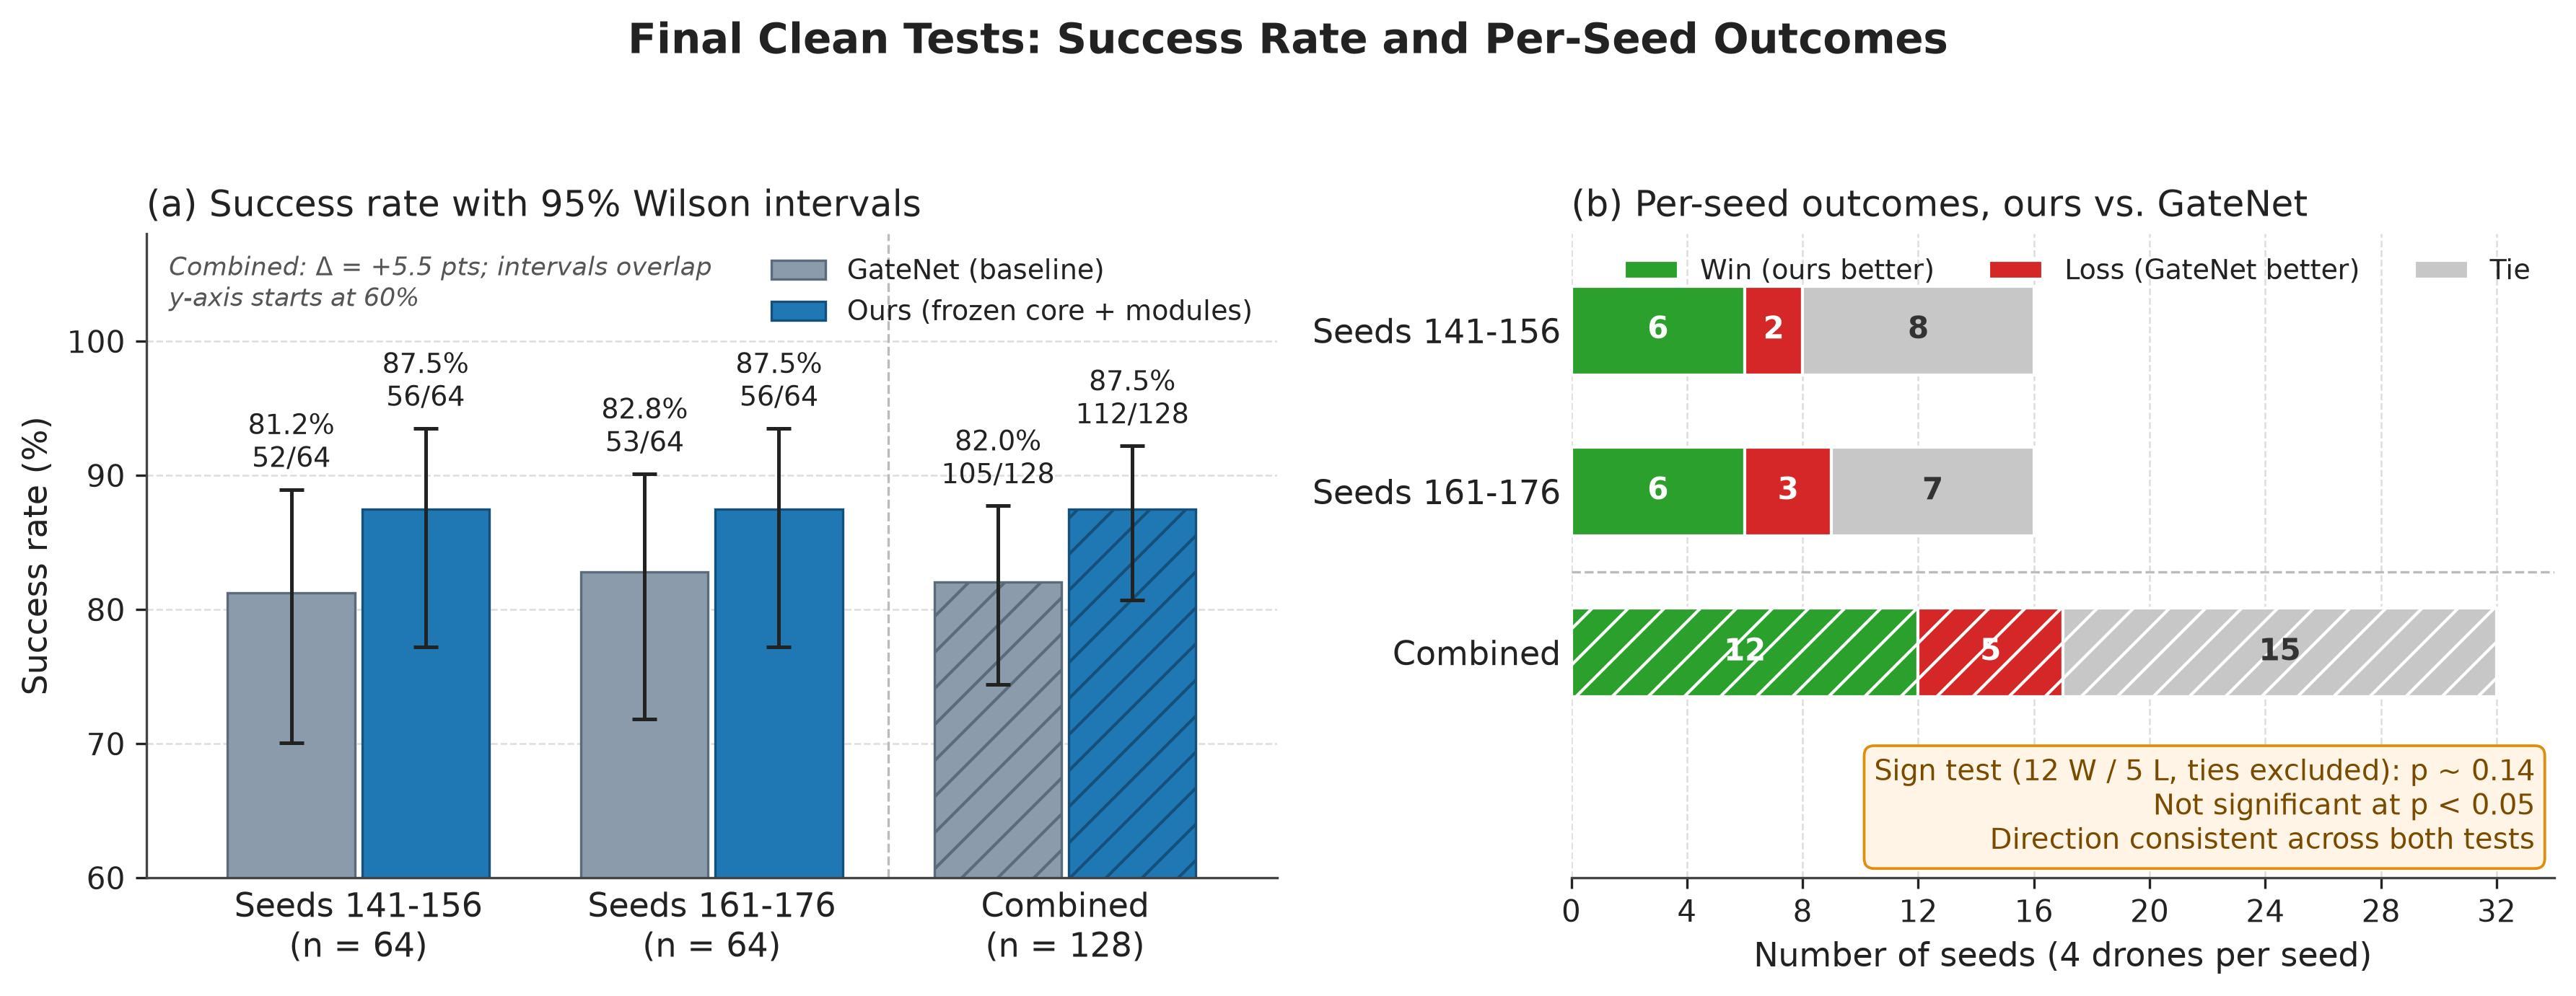
\includegraphics[width=\linewidth]{figures/fig_final_clean_test_success_and_seed_outcomes.jpg}
  \caption{Final tests in simulation (seeds 141--156 and 161--176, 64 flights per arm per test). \textbf{(a)} Success rates with 95\% Wilson intervals and success counts. Ours reaches 87.5\% in both tests, against 81.2\% and 82.8\% for GateNet, and 87.5\% against 82.0\% over all 128 flights (+5.5 points). The intervals overlap, and the y-axis starts at 60\%. \textbf{(b)} Per-seed outcomes (wins/losses/ties: 6/2/8, 6/3/7; 12/5/15 combined; hatched bars are combined). The sign test gives $p\approx0.14$. The direction is consistent but not significant at $p<0.05$.}
  \label{fig:clean}
\end{figure}

\Cref{tab:main} and \cref{fig:clean} summarize the final comparison. In both independent final tests our system completes 56 of 64 flights (87.5\%). GateNet completes 52/64 (81.2\%) and 53/64 (82.8\%). Over all 128 flights per arm this gives 87.5\% versus 82.0\%, a difference of 5.5 points. At the seed level, our arm wins 12 seeds, loses 5 and ties 15. A two-sided sign test on the 17 non-tied seeds gives $p\approx0.14$. The difference has the same sign in both tests and in both the flight-level and seed-level counts, but it is \emph{not} statistically significant at $p<0.05$, and the Wilson intervals in \cref{fig:clean}a overlap. We therefore claim that the frozen core with modules \emph{matches} the dedicated detector in this loop. We do not claim superiority. Both arms fly at a path speed of about 19\,m/s. An example flight of our arm passes all 22 gates with a 17.4\,s lap.

\begin{table}[t]
  \centering
  \small
  \setlength{\tabcolsep}{3pt}
  \begin{tabular}{@{}lcccc@{}}
    \toprule
    & \multicolumn{2}{c}{Test 1 (141--156)} & \multicolumn{2}{c}{Test 2 (161--176)} \\
    \cmidrule(lr){2-3}\cmidrule(l){4-5}
    Distance & GateNet & Ours & GateNet & Ours \\
    \midrule
    0--2\,m & 0.096/0.206 & 0.088/0.210 & 0.089/0.225 & 0.084/0.198 \\
    2--4\,m & 0.111/0.351 & 0.107/0.272 & 0.107/0.407 & 0.103/0.258 \\
    4--8\,m & 0.129/0.367 & 0.130/0.301 & 0.124/0.344 & 0.124/0.279 \\
    8+\,m & 0.212/0.500 & 0.241/0.606 & 0.204/0.458 & 0.242/0.571 \\
    \bottomrule
  \end{tabular}
  \caption{EKF next-gate position error (median/p90, metres) binned by true distance to the gate, on both final tests.}
  \label{tab:ekf}
\end{table}

\begin{figure}[t]
  \centering
  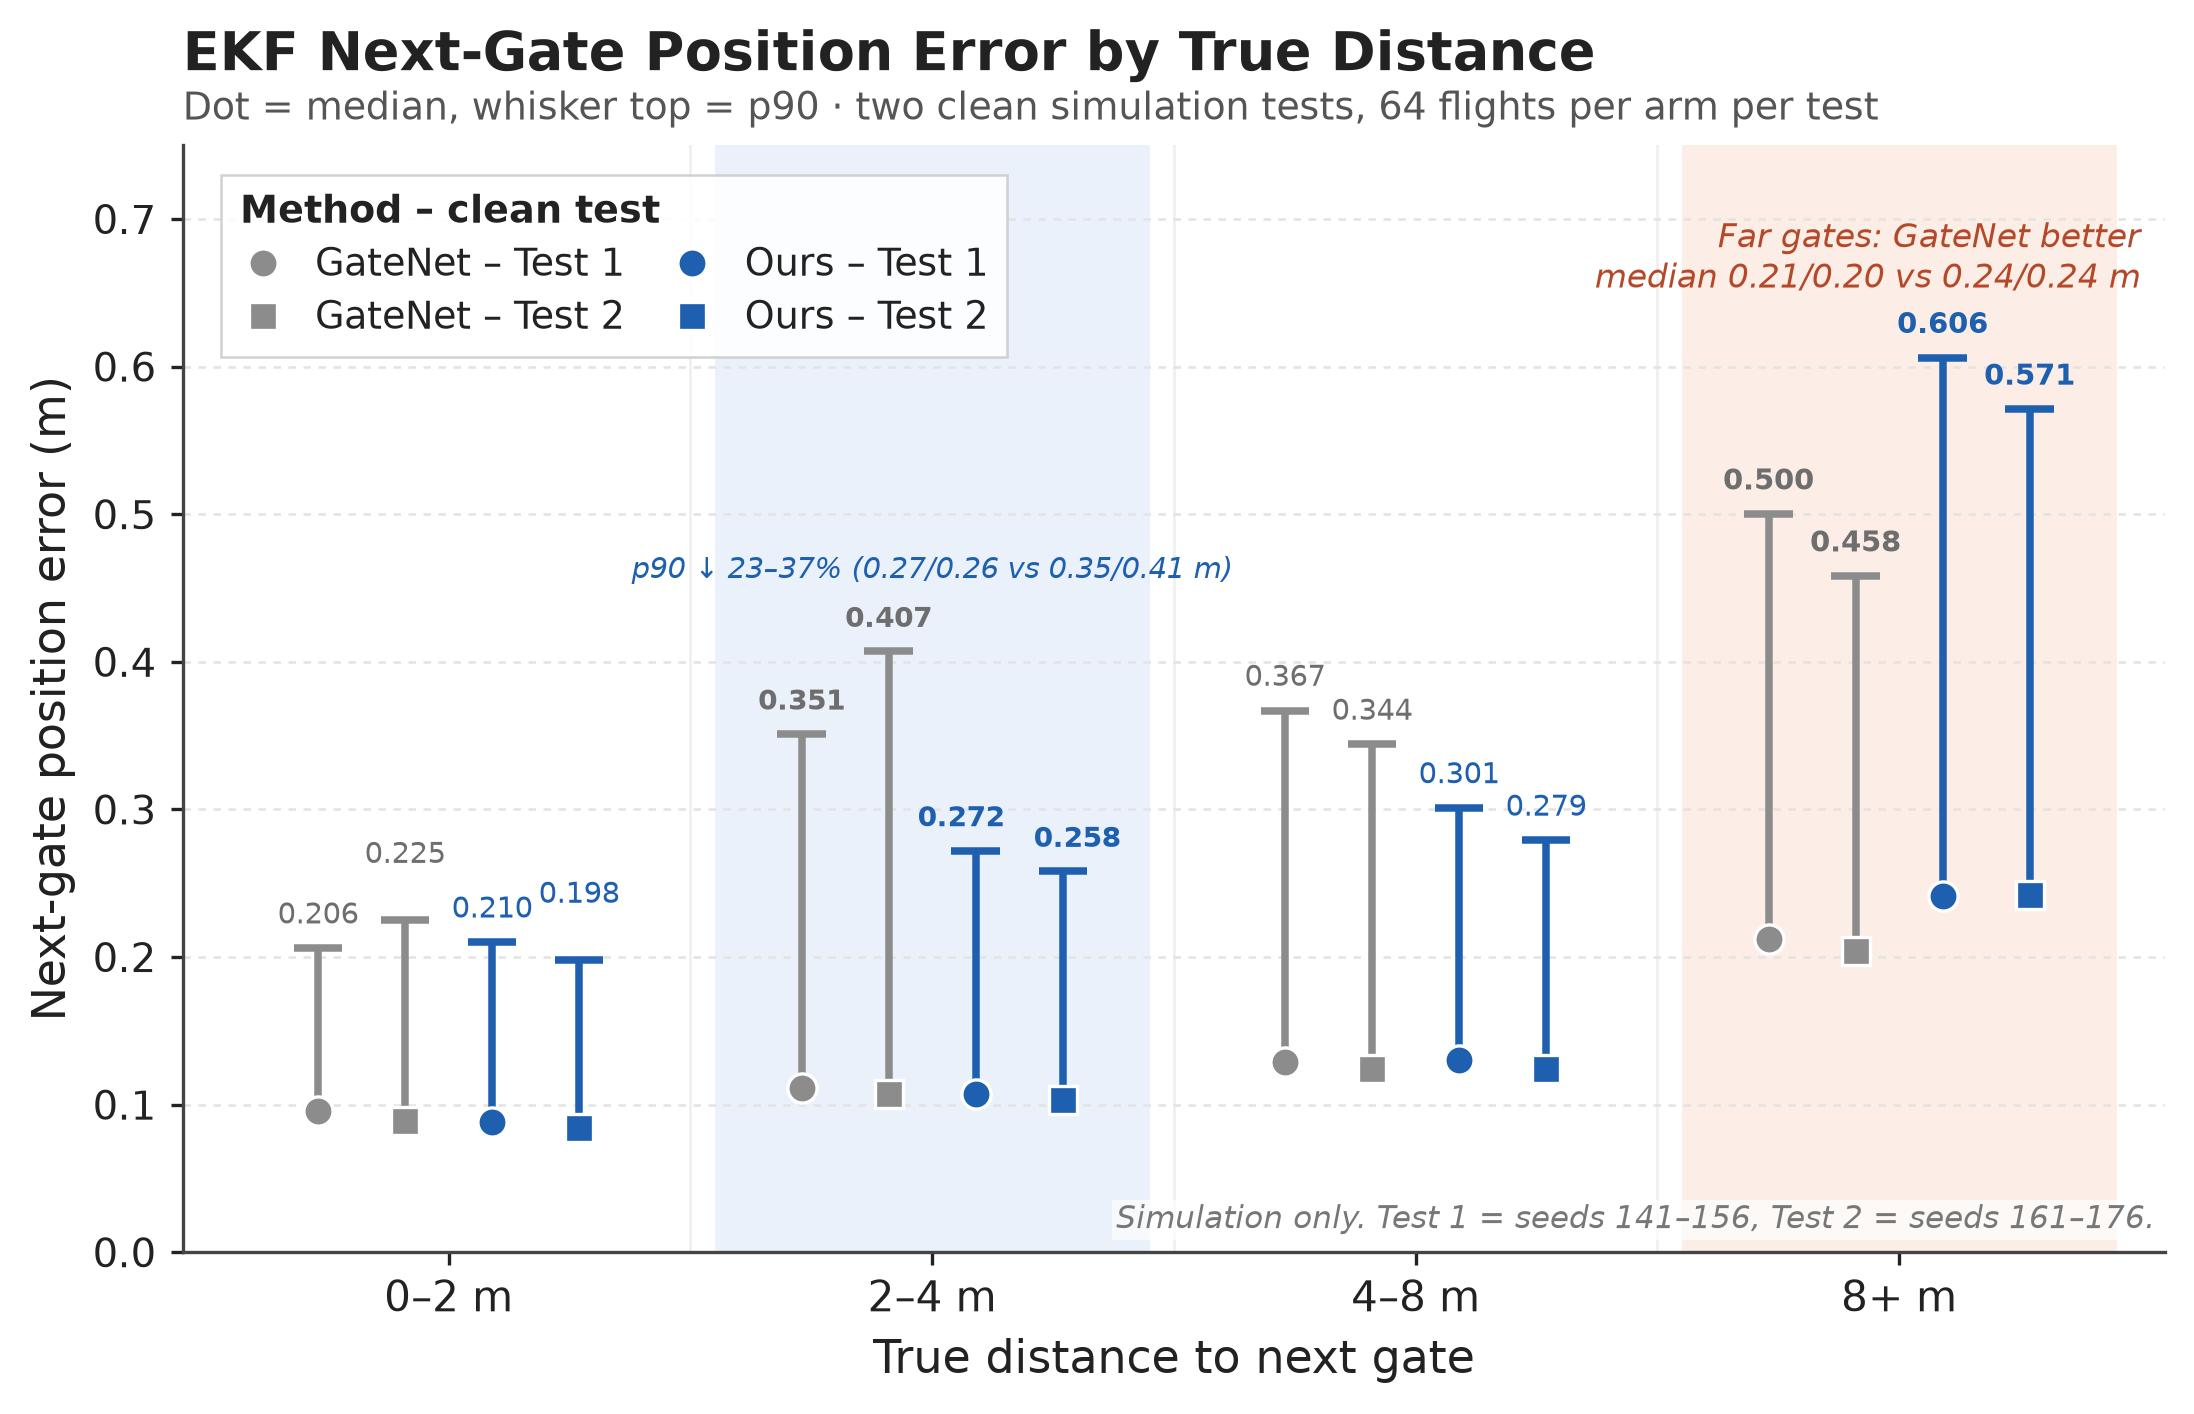
\includegraphics[width=\linewidth]{figures/fig_estimator_error_by_distance.jpg}
  \caption{EKF next-gate position error by true distance, GateNet (grey) vs.\ ours (blue), on Test 1 (seeds 141--156, circles) and Test 2 (seeds 161--176, squares). Markers show medians; whiskers extend to p90. Up to 8\,m the medians nearly coincide (0.08--0.13\,m), but our p90 is lower. At 2--4\,m it is 0.27/0.26\,m against 0.35/0.41\,m, a reduction of about 23--37\%. For far gates (8+\,m) GateNet is better, with lower medians (0.21/0.20 vs.\ 0.24/0.24\,m) and shorter tails (p90 0.50/0.46 vs.\ 0.61/0.57\,m).}
  \label{fig:ekf}
\end{figure}

\paragraph{Estimator error.}
\Cref{tab:ekf} and \cref{fig:ekf} show where the arms differ. Up to 8\,m, the median next-gate errors of both arms are almost identical (0.084--0.130\,m). The difference lies in the tails. At 2--4\,m our p90 error is 0.272/0.258\,m versus 0.351/0.407\,m for GateNet, and at 4--8\,m it is 0.301/0.279\,m versus 0.367/0.344\,m. Large estimator errors at near and mid range are the ones most likely to cause a crash at the next gate, which is consistent with the success rates. For far gates (8+\,m) the picture reverses. GateNet has lower medians (0.212/0.204 vs.\ 0.241/0.242\,m) and shorter tails (0.500/0.458 vs.\ 0.606/0.571\,m). Two mechanisms plausibly contribute. First, far gates project to small boxes, and the min14 filter, chosen to maximize validation success, removes some of these observations, so the EKF relies more on its map prior. Second, for the small far gates that remain, the core's coarse stride-4 corners carry less precise information than at near range. The filter thus trades far-gate observations for fewer unreliable small detections. On balance this raised success on validation seeds (\cref{sec:ablation}), but it shows up as larger far-range error.

\subsection{General capabilities are preserved}
\label{sec:general}
\begin{table}[t]
  \centering
  \small
  \begin{tabular}{@{}llc@{}}
    \toprule
    Task / set & Metric & Value \\
    \midrule
    Gates, red (never seen) & within 20 / 10\,px & 0.987 / 0.958 \\
    Gates, red, nested & found & 20 / 20 \\
    Gates, TII flight video & within 20\,px & 0.962 \\
    Seg.\ false-gate frames, red & rate & 0.026 \\
    Lane, TuSimple & IoU & 0.803 \\
    Seg., SUN RGB-D & mIoU & 0.749 \\
    Seg., BDD100K (sky-aware) & mIoU & 0.734 \\
    Seg., ADE20K (subset) & mIoU & 0.595 \\
    Seg., IDD-AW & mIoU & 0.609 \\
    Seg., RUGD (held-out) & mIoU & 0.505 \\
    Seg., Aeroscapes (drone) & IoU & 0.614 \\
    \bottomrule
  \end{tabular}
  \caption{General metrics of the frozen core (release v4, 448\,px). Gate rows refer to the core's own gate head. These values are identical with and without the plug-in modules (\cref{eq:nonregression}).}
  \label{tab:general}
\end{table}

\Cref{tab:general} lists the general metrics of the frozen core. Because the modules never modify $\theta$, every value holds with and without them. The core places 0.987 of corners within 20\,px and 0.958 within 10\,px at the never-seen real place, finds all 20 nested gates there, and reaches 0.962 within 20\,px on a real flight video. Lane IoU on TuSimple is 0.803. Segmentation mIoU ranges from 0.505 on held-out off-road RUGD to 0.749 on SUN RGB-D.

To put these values in context, we trained three 16-epoch seeds of the core. Red within 10\,px varied between 0.939 and 0.958, and lane IoU between 0.803 and 0.804. The Aeroscapes drone IoU was noisy (0.539--0.675). Any retraining of the core, as in the attempts of \cref{sec:ablation}, therefore moves general metrics by amounts at least comparable to this seed variation and requires re-validating all benchmarks. Read-only extension avoids both.

At the never-seen real place, GateNet places 0.776 of corners within 20\,px, versus 0.987 for the core's gate head. This comparison should be read narrowly. It measures the core's gate head, \ie the input on which the modules build, not the full module pipeline. It also contrasts a model whose training data include real gates with a detector trained only on simulator data. It therefore reflects the breadth of the core's training data rather than a matched comparison of the two architectures. Its relevance here is that the real-gate ability of the released core is retained unchanged when modules are added.

\subsection{Diagnosis and ablations: from 37.5\% to 87.5\%}
\label{sec:ablation}
\begin{figure*}[t]
  \centering
  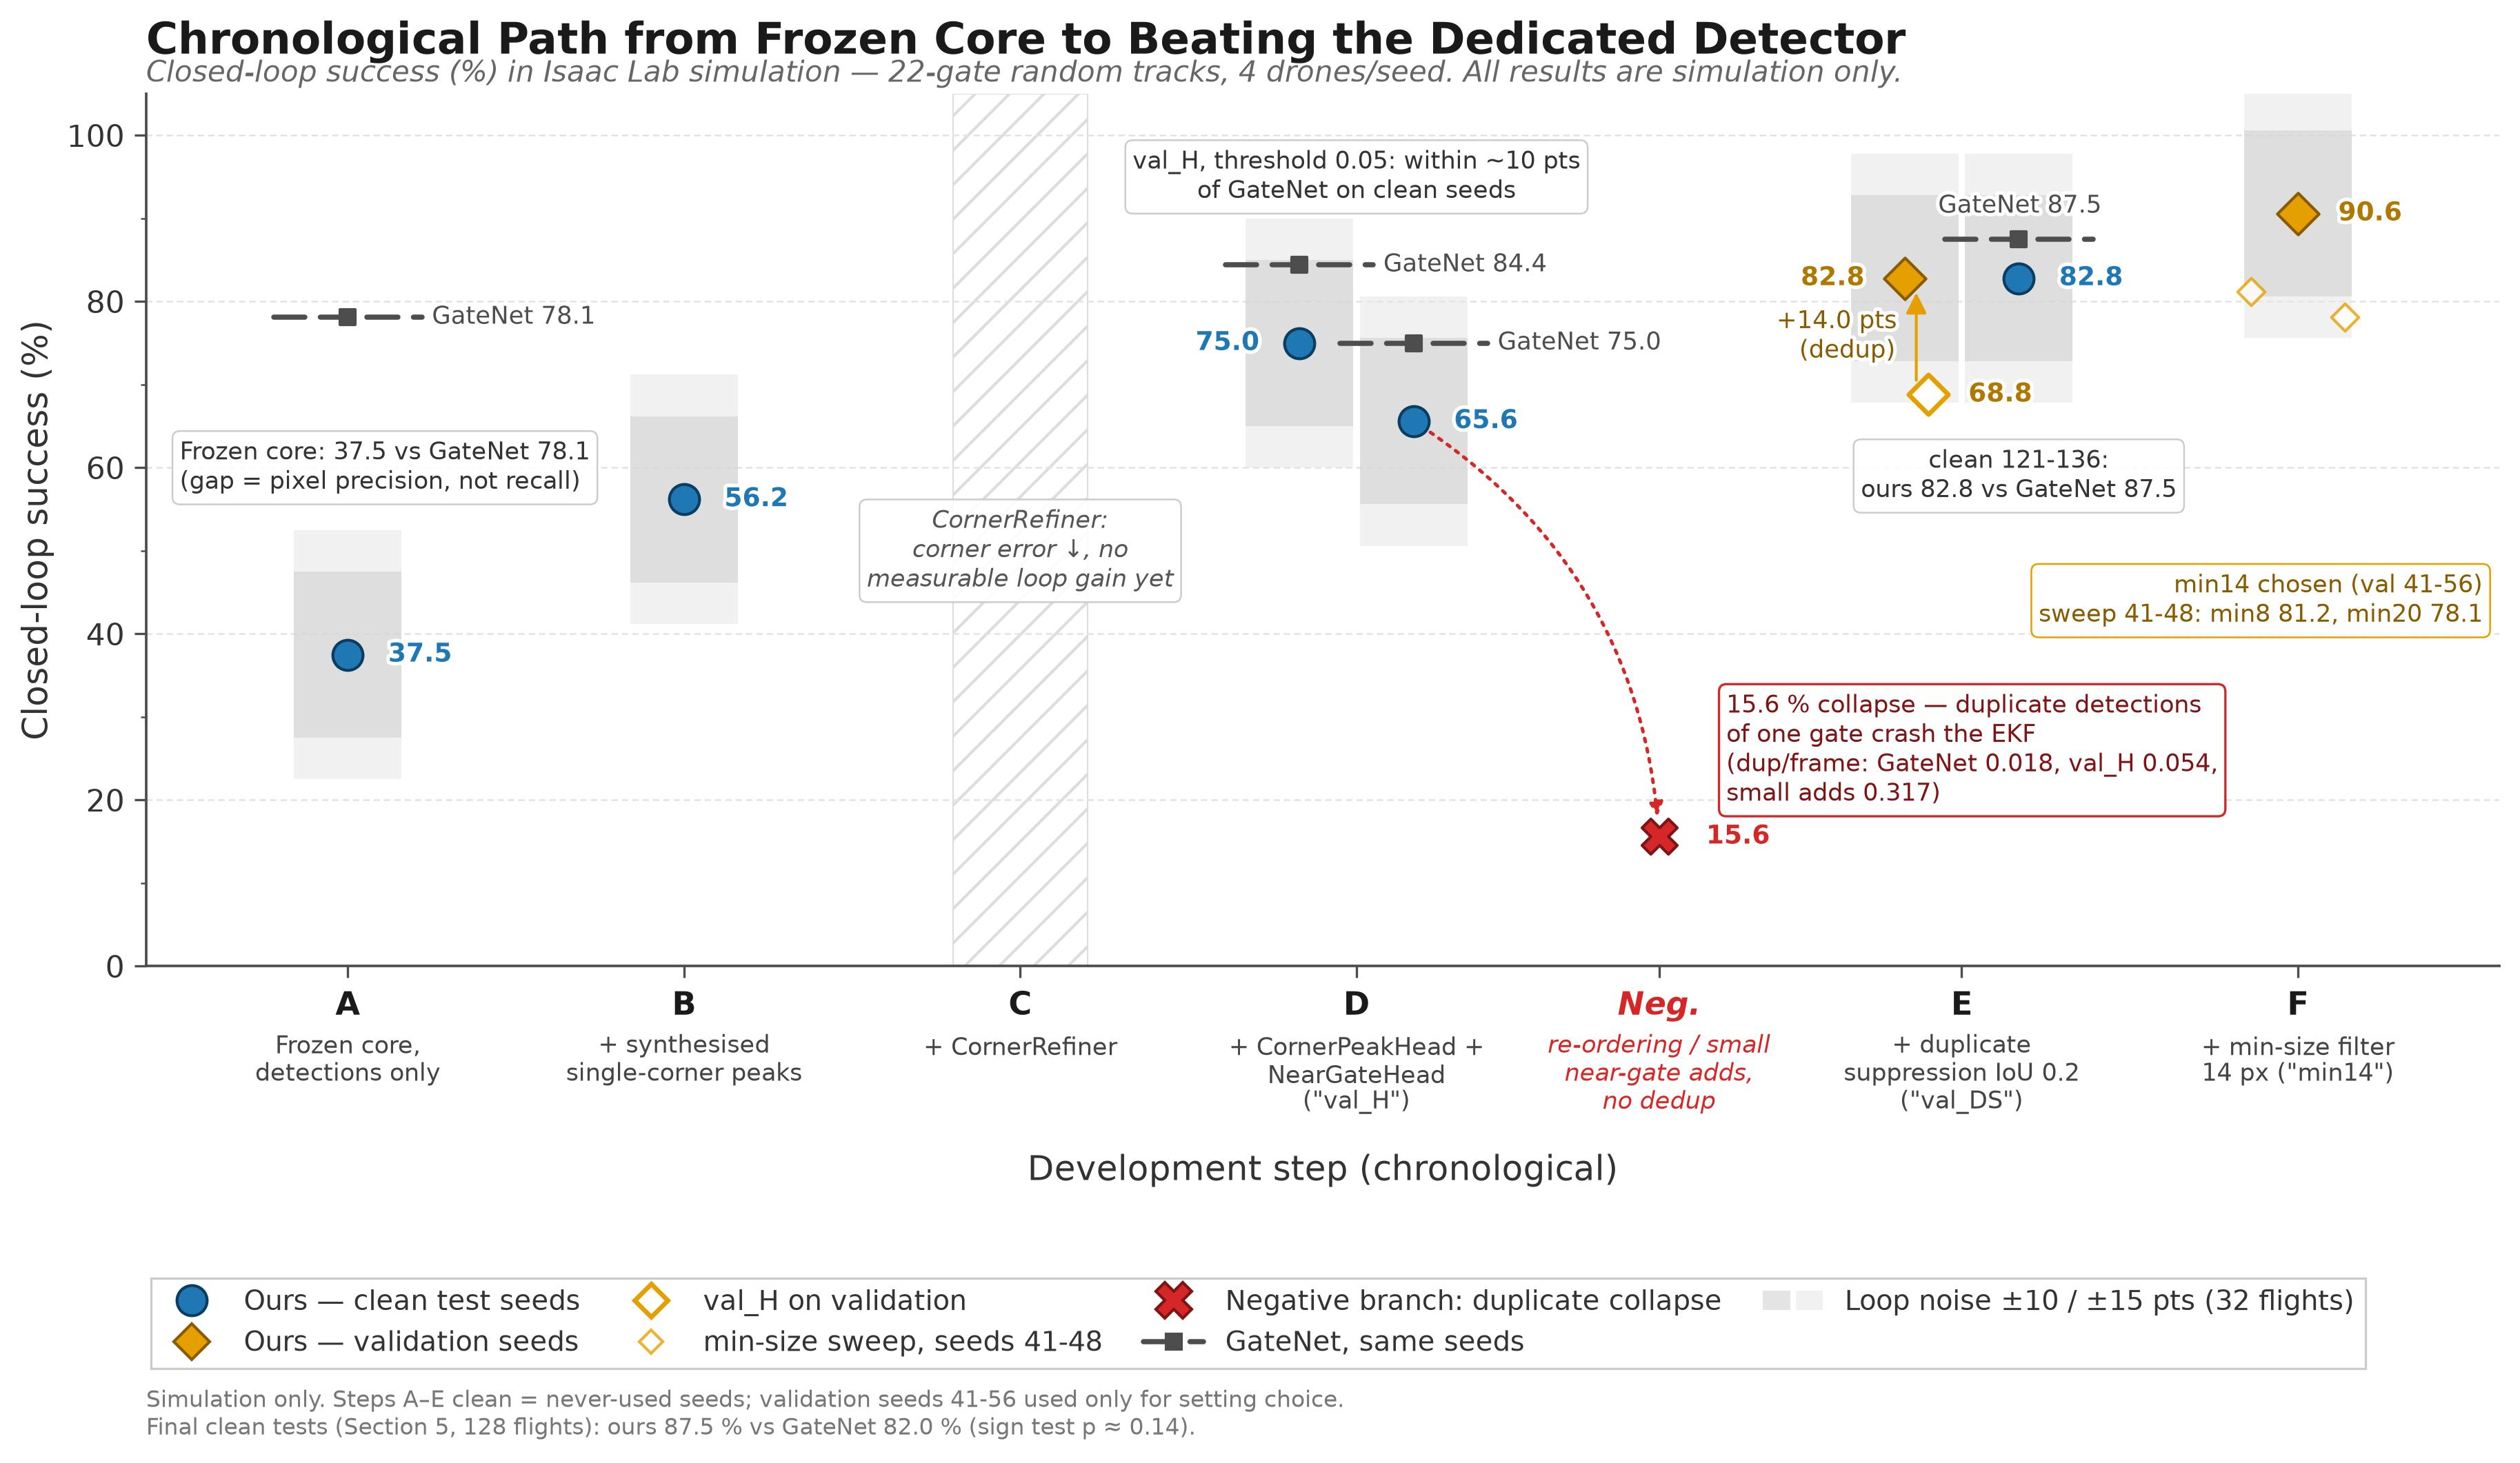
\includegraphics[width=\textwidth]{figures/fig_development_path_success_rate_progression.jpg}
  \caption{Closed-loop success (\%) of the frozen-core detector at each development step (A--F), in Isaac Lab simulation only. Blue circles are development-check seeds, each evaluated once on fresh tracks after a step; filled orange diamonds are validation seeds 41--56. Hollow diamonds show val\_H on the same validation seeds and the min-size sweep (min8, min20) on seeds 41--48. Dashed grey segments show GateNet wherever it was evaluated on the same seeds. Grey bands mark loop noise of $\pm$10 and $\pm$15 points for 32 flights. Starting from 37.5\% against GateNet's 78.1\% (A), synthesised corner peaks (B), the CornerRefiner (C, no measurable loop gain) and the CornerPeakHead and NearGateHead (D) narrow the gap to about 10 points. Adding small near-gate detections without deduplication collapses success to 15.6\%. Global duplicate suppression (E) adds 14.0 points on validation and reaches 82.8\% against GateNet's 87.5\% on seeds 121--136. The 14\,px minimum-size filter (F) reaches 90.6\% on validation.}
  \label{fig:path}
\end{figure*}

\begin{table}[t]
  \centering
  \small
  \setlength{\tabcolsep}{3pt}
  \begin{tabular}{@{}llcc@{}}
    \toprule
    Step & Seeds (role) & GateNet & Ours \\
    \midrule
    A: frozen core & 71--78 (dev.) & 78.1 & 37.5 \\
    B: + corner peaks & dev. & -- & 56.2 \\
    C: + CornerRefiner & -- & -- & no loop gain \\
    D: + cpk3, ng2 (val\_H) & 91--98 (dev.) & 84.4 & 75.0 \\
     & 101--116 (dev.) & 75.0 & 65.6 \\
     & 41--56 (val) & -- & 68.8 \\
    Neg.: small adds, no dedup & -- & -- & 15.6 \\
    E: + dup.\ supp.\ (val\_DS) & 41--56 (val) & -- & 82.8 \\
     & 121--136 (dev.) & 87.5 & 82.8 \\
    F: + min14 & 41--56 (val) & -- & 90.6 \\
    \midrule
    Final & 141--176 (test) & 82.0 & 87.5 \\
    \bottomrule
  \end{tabular}
  \caption{Chronological, cumulative development path (closed-loop success, \%). dev.: development-check seeds; val: validation; test: final-test seeds. ``--'' indicates not measured on the same seeds or not reported.}
  \label{tab:path}
\end{table}

\Cref{fig:path} and \cref{tab:path} trace the development path. Each step was motivated by an in-loop diagnosis rather than by offline scores. The path is cumulative: each step adds to the previous configuration. Step-wise results use 32--64 flights, so individual step differences, apart from the large changes at A$\to$D and the collapse to 15.6\%, lie within loop noise. We read them as qualitative guidance. Only the final tests (\cref{sec:main}) support a quantitative comparison.

\paragraph{Step A: the frozen core alone is not enough.}
Using only the core's gate head, our arm succeeded in 37.5\% of flights versus 78.1\% for GateNet (seeds 71--78), despite the core's strong offline accuracy on real gates (\cref{sec:general}).

\begin{figure}[t]
  \centering
  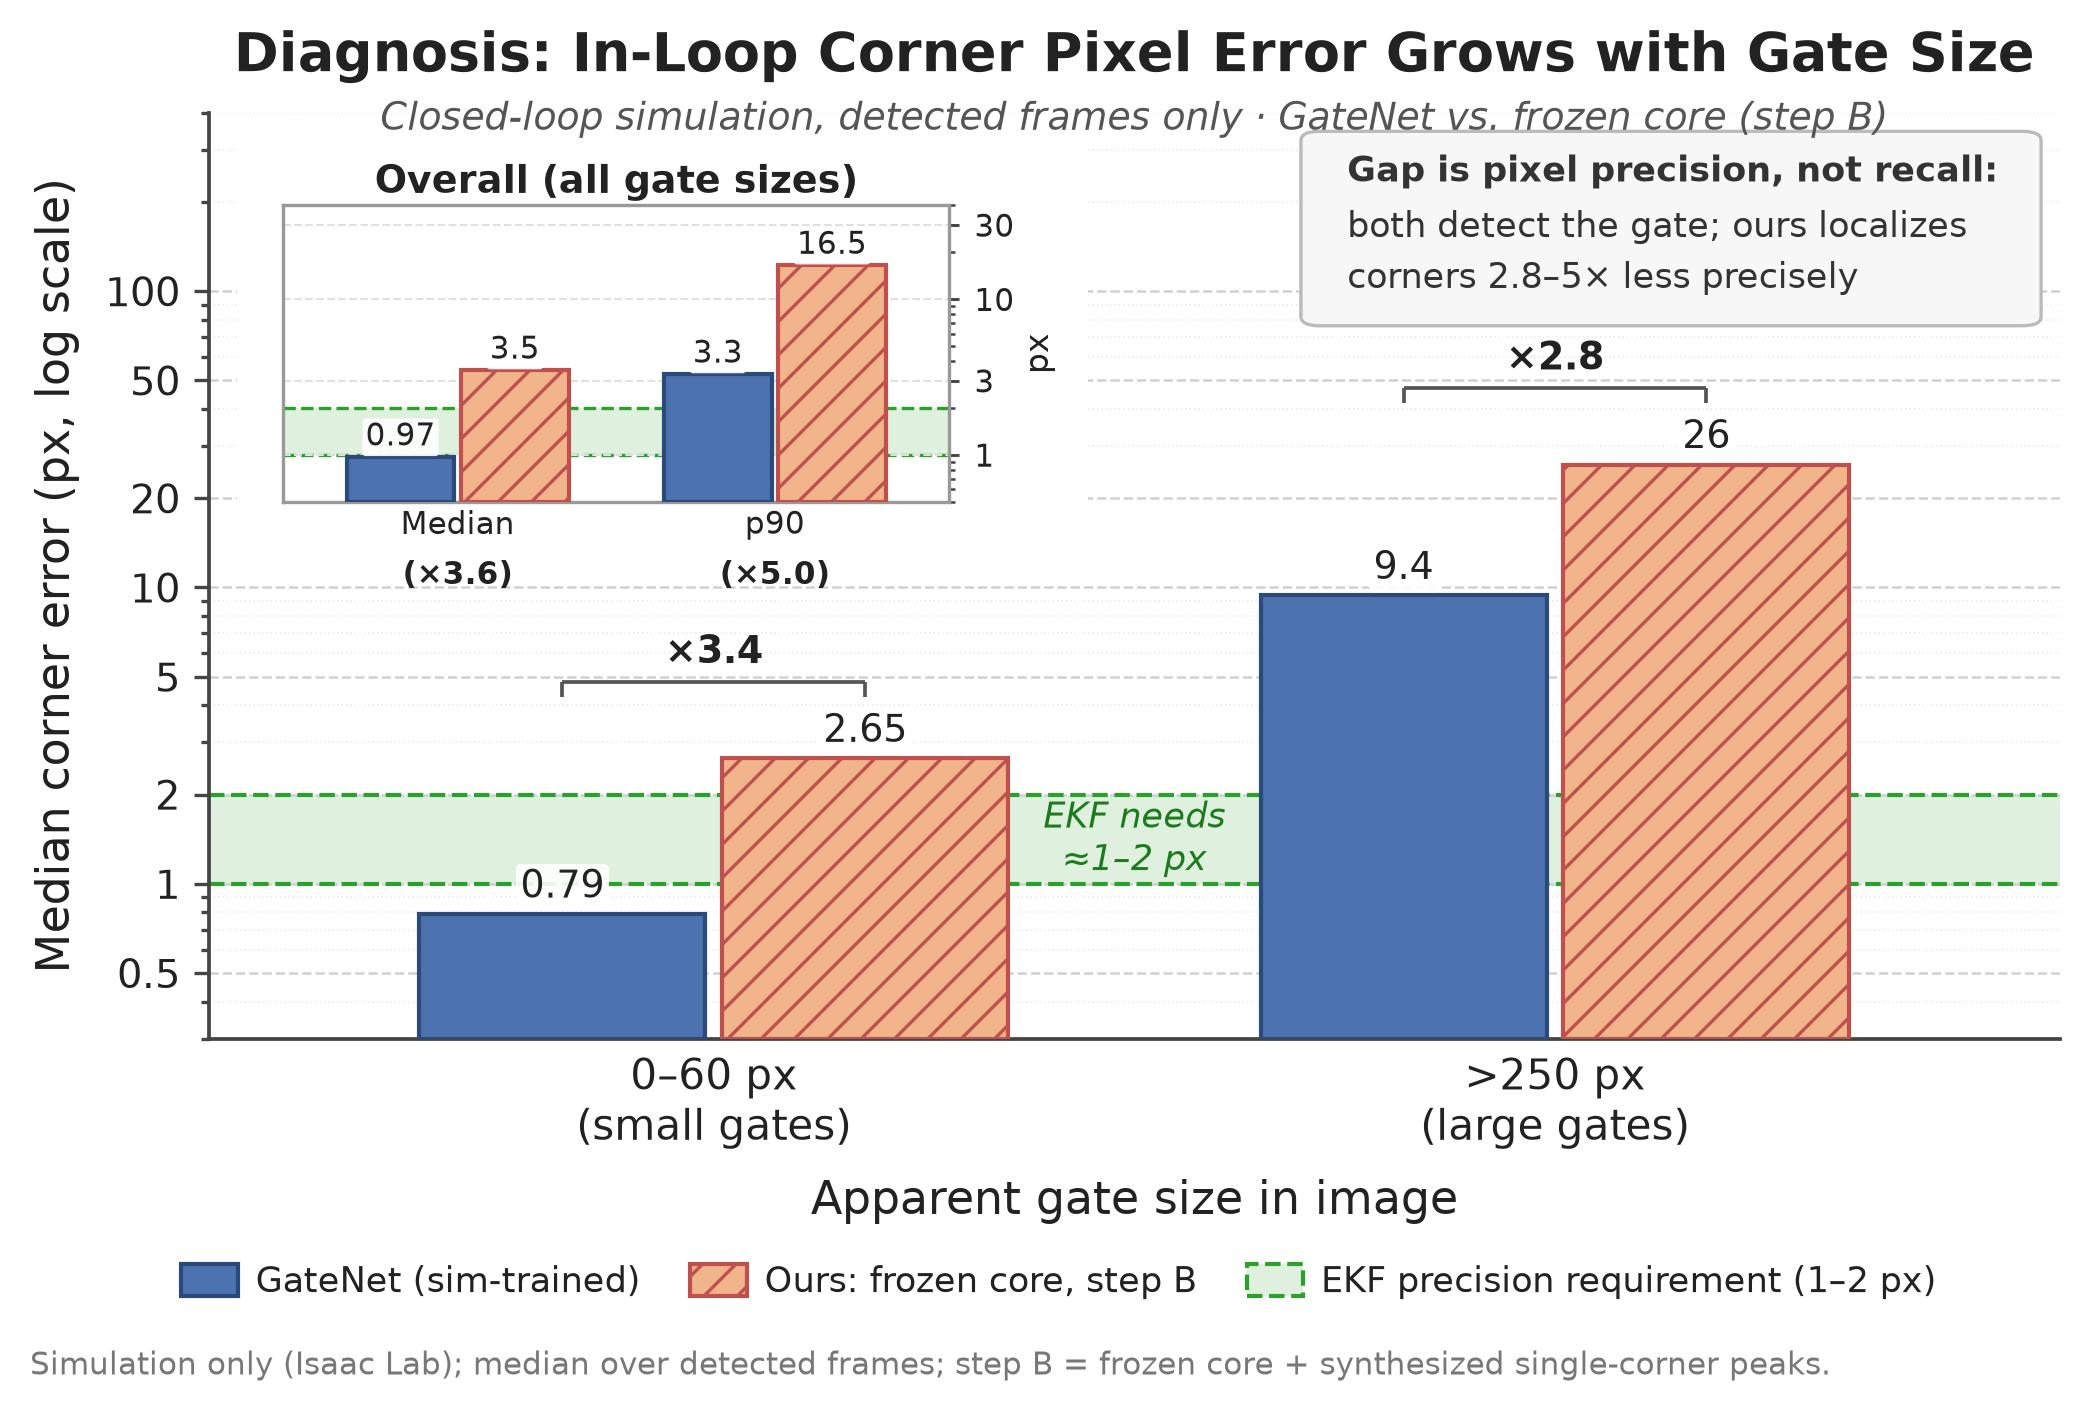
\includegraphics[width=\linewidth]{figures/fig_incloop_corner_error_vs_gate_size.jpg}
  \caption{Median in-loop corner error (px, log scale) for detected frames only, GateNet (solid blue) vs.\ our frozen core at step B (hatched orange), in closed-loop simulation. For small gates (0--60\,px) the errors are 0.79 vs.\ 2.65\,px ($\times$3.4); for large gates ($>$250\,px), 9.4 vs.\ 26\,px ($\times$2.8). Inset: overall median 0.97 vs.\ 3.5\,px ($\times$3.6) and p90 3.3 vs.\ 16.5\,px ($\times$5.0). The green band marks the $\sim$1--2\,px precision required by the EKF. Both detectors find the gate in these frames, so the gap comes from precision, not recall.}
  \label{fig:cornererr}
\end{figure}

\paragraph{Diagnosis: precision, not recall.}
After step B (synthesised single-corner peaks, 56.2\%), we measured the corner error inside the loop on frames where both detectors found the gate (\cref{fig:cornererr}). GateNet's median error was 0.97\,px (p90 3.3\,px), ours was 3.5\,px (p90 16.5\,px). The gap was present for small gates (0.79 vs.\ 2.65\,px) and largest in absolute terms for frame-filling gates (9.4 vs.\ 26\,px above 250\,px). The EKF needs roughly 1--2\,px. GateNet's small-gate error lies inside this band, while our step-B errors lie above it in every size bin. Since both detectors find the gate in these frames, the closed-loop gap is due to pixel precision and not to recall. This diagnosis motivates the CornerRefiner (sub-pixel precision) and the NearGateHead (large gates).

\paragraph{Negative result: changing the core did not help.}
Before adopting modules, we tried to obtain precision inside the core. We retrained or fine-tuned it on simulator renders, raised the corner loss weight to 10, 40 and 100, used a stride-2 dense corner head, and averaged weights into model soups. In our closed-loop checks none of these produced a gain beyond loop noise, and the general-metric cost grew with the corner weight. We report these attempts qualitatively. Their practical implication is that each would also have required re-validating a new core on all benchmarks of \cref{tab:general}, without a demonstrated benefit for the target. We therefore kept the core frozen.

\paragraph{Steps C and D: modules.}
The CornerRefiner (C) improved corner accuracy, but the loop did not yet improve measurably. Precision alone was not enough while weak and near gates were still missed or poorly localized. Adding the CornerPeakHead, which allows the detection threshold to drop to 0.05, and the NearGateHead (D, val\_H) brought the system to about 10 points of GateNet on development-check seeds: 75.0 vs.\ 84.4 (seeds 91--98) and 65.6 vs.\ 75.0 (seeds 101--116). Its isolated contribution in the final configuration is not separated by our cumulative path. We retain the CornerRefiner because it addresses the bottleneck identified by the diagnosis: its sub-pixel corrections apply to every core detection that the later steps keep.

\begin{figure}[t]
  \centering
  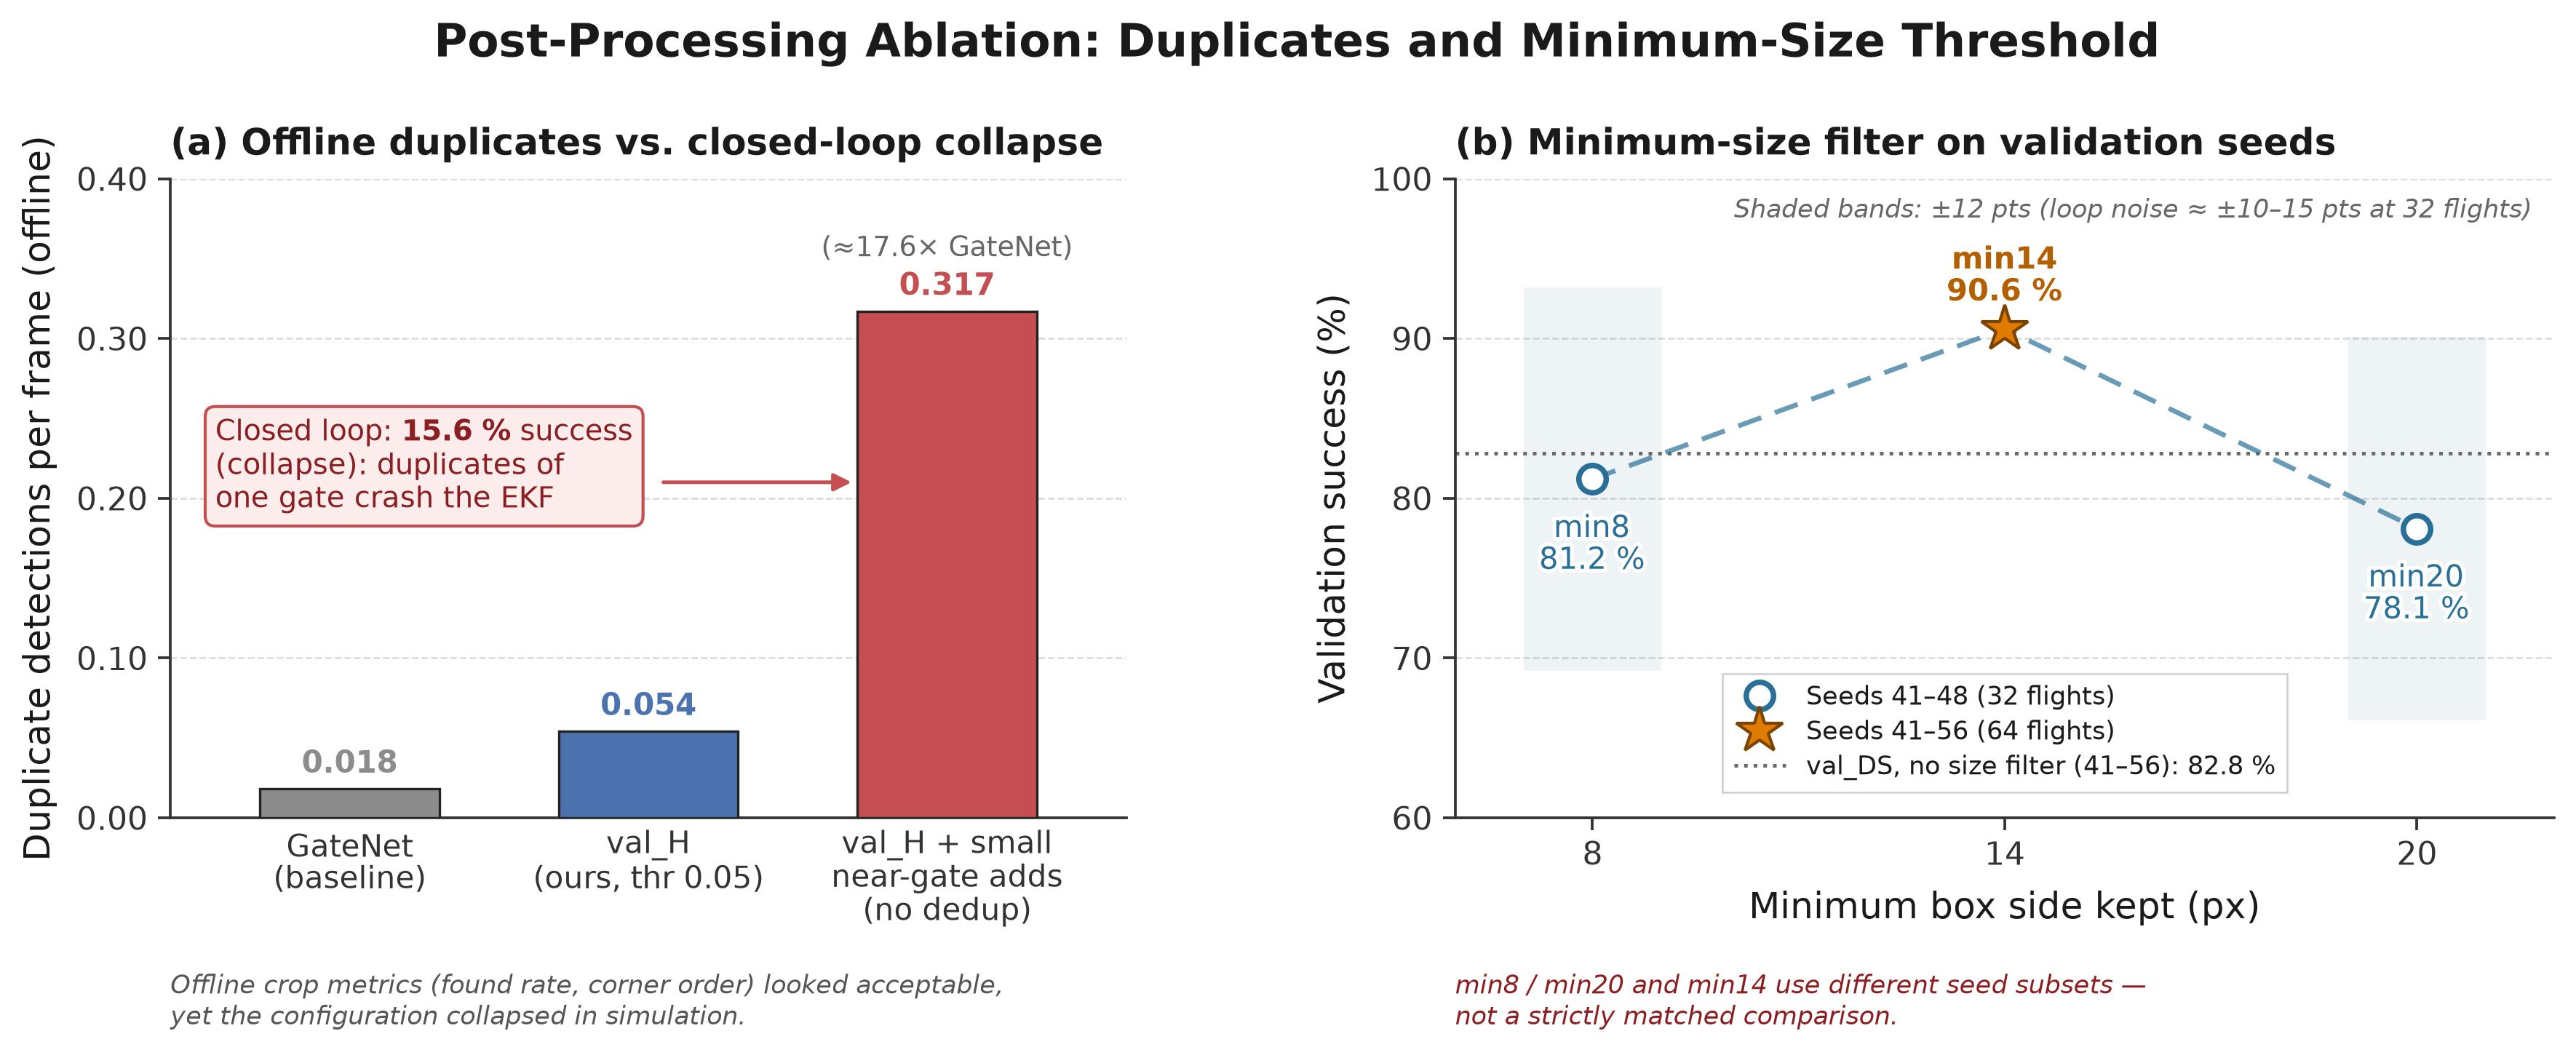
\includegraphics[width=\linewidth]{figures/fig_ablation_duplicates_and_min_size_filter.jpg}
  \caption{Post-processing ablation in closed-loop simulation. \textbf{(a)} Offline duplicate detections per frame: GateNet 0.018, val\_H 0.054, and 0.317 ($\approx$17.6$\times$ GateNet) after adding small near-gate detections without deduplication. In closed loop that configuration collapsed to 15.6\% success, although offline found rate and corner order looked acceptable. \textbf{(b)} Validation success vs.\ minimum box side. min14 (star) reached 90.6\% on seeds 41--56 (64 flights); min8 and min20 reached 81.2\% and 78.1\% on the subset 41--48 (32 flights), so the comparison is not strictly matched. The dotted line marks val\_DS without a size filter (82.8\%, seeds 41--56). Shaded bands show $\pm$12 points.}
  \label{fig:ablation}
\end{figure}

\paragraph{Negative result: duplicates collapse the loop.}
Three variants that looked reasonable offline were catastrophic in the loop: re-ordering corners to an identity order, geometrically sorting near-gate detections, and adding small near-gate detections without deduplication. Success collapsed to 15.6\%. Offline, duplicates per frame were 0.018 for GateNet, 0.054 for val\_H and 0.317 with the small adds (\cref{fig:ablation}a), while found rate and corner order did not reveal the problem. When one gate is reported twice, the EKF receives inconsistent observations of the same landmark and diverges. This is a known data-association hazard for landmark-based filters. Our observation is narrower than a general claim about offline--online correlation: in this loop, the offline crop metrics we tracked (found rate, order) did not flag this hazard, whereas the duplicate rate did.

\paragraph{Steps E and F: post-processing.}
Global duplicate suppression at IoU 0.2 (E, val\_DS) raised validation success on seeds 41--56 from 68.8\% (val\_H) to 82.8\%, a gain of 14.0 points. On development-check seeds 121--136 it reached 82.8\% versus GateNet's 87.5\%, which is within loop noise. The minimum-size filter (F) was swept on validation seeds (\cref{fig:ablation}b). min14 reached 90.6\% on seeds 41--56, while min8 (81.2\%) and min20 (78.1\%) were evaluated on the smaller subset 41--48. This comparison is not strictly matched and every point lies within about $\pm$12 points of noise. We read it only as evidence that a moderate threshold is preferable: very small boxes give unreliable corners, while a large threshold discards useful far-gate observations. min14 was fixed before the final tests.

\paragraph{Attribution of the post-processing.}
Both steps are parameter-free and could, in principle, be applied to any detector. Duplicate suppression, however, mainly addresses a failure created by our own pipeline. It merges detections from three sources, and val\_H produced 0.054 duplicates per frame against 0.018 for GateNet, so GateNet's single-source output leaves far less for this step to remove. The min-size filter is a generic step whose effect on GateNet was not part of our protocol. The gains of E and F should therefore be read as making the multi-source module pipeline compatible with the estimator, on top of the precision provided by the modules (steps B--D, 37.5$\to$75.0\% on development-check seeds 91--98).

\paragraph{Lessons.}
Three observations summarize the path. (i) In-loop precision, measured in pixels on the frames the estimator actually consumes, was the limiting factor, not offline recall. (ii) The interface to the downstream consumer matters: in this loop one duplicate per gate was more harmful than any corner error we observed. (iii) All improvements came from read-only heads and parameter-free post-processing, never from changing the core, so none of them required re-validating the general model.

\subsection{Edge deployment}
\label{sec:edge}
\begin{table}[t]
  \centering
  \small
  \setlength{\tabcolsep}{3pt}
  \begin{tabular}{@{}lccc@{}}
    \toprule
    Model & 15\,W ms (FPS) & MAXN ms (FPS) & J/frame \\
    \midrule
    ViT-B (87.7M) & 39.5 (25.3) & 19.6 (50.9) & 0.482$\to$0.348 \\
    Hybrid, plain & 44.2 (22.6) & 24.7 (40.5) & 0.465$\to$0.377 \\
    Hybrid, reparam. & \textbf{26.4} (37.9) & \textbf{14.6} (68.7) & \textbf{0.286}$\to$\textbf{0.230} \\
    \bottomrule
  \end{tabular}
  \caption{Core latency (median) and total energy per frame (15\,W$\to$MAXN) on Jetson Orin NX 8\,GB, TensorRT fp16, 384$\times$384, batch 1, GPU compute only. Module latency on the Orin has not yet been measured.}
  \label{tab:edge}
\end{table}

\begin{figure}[t]
  \centering
  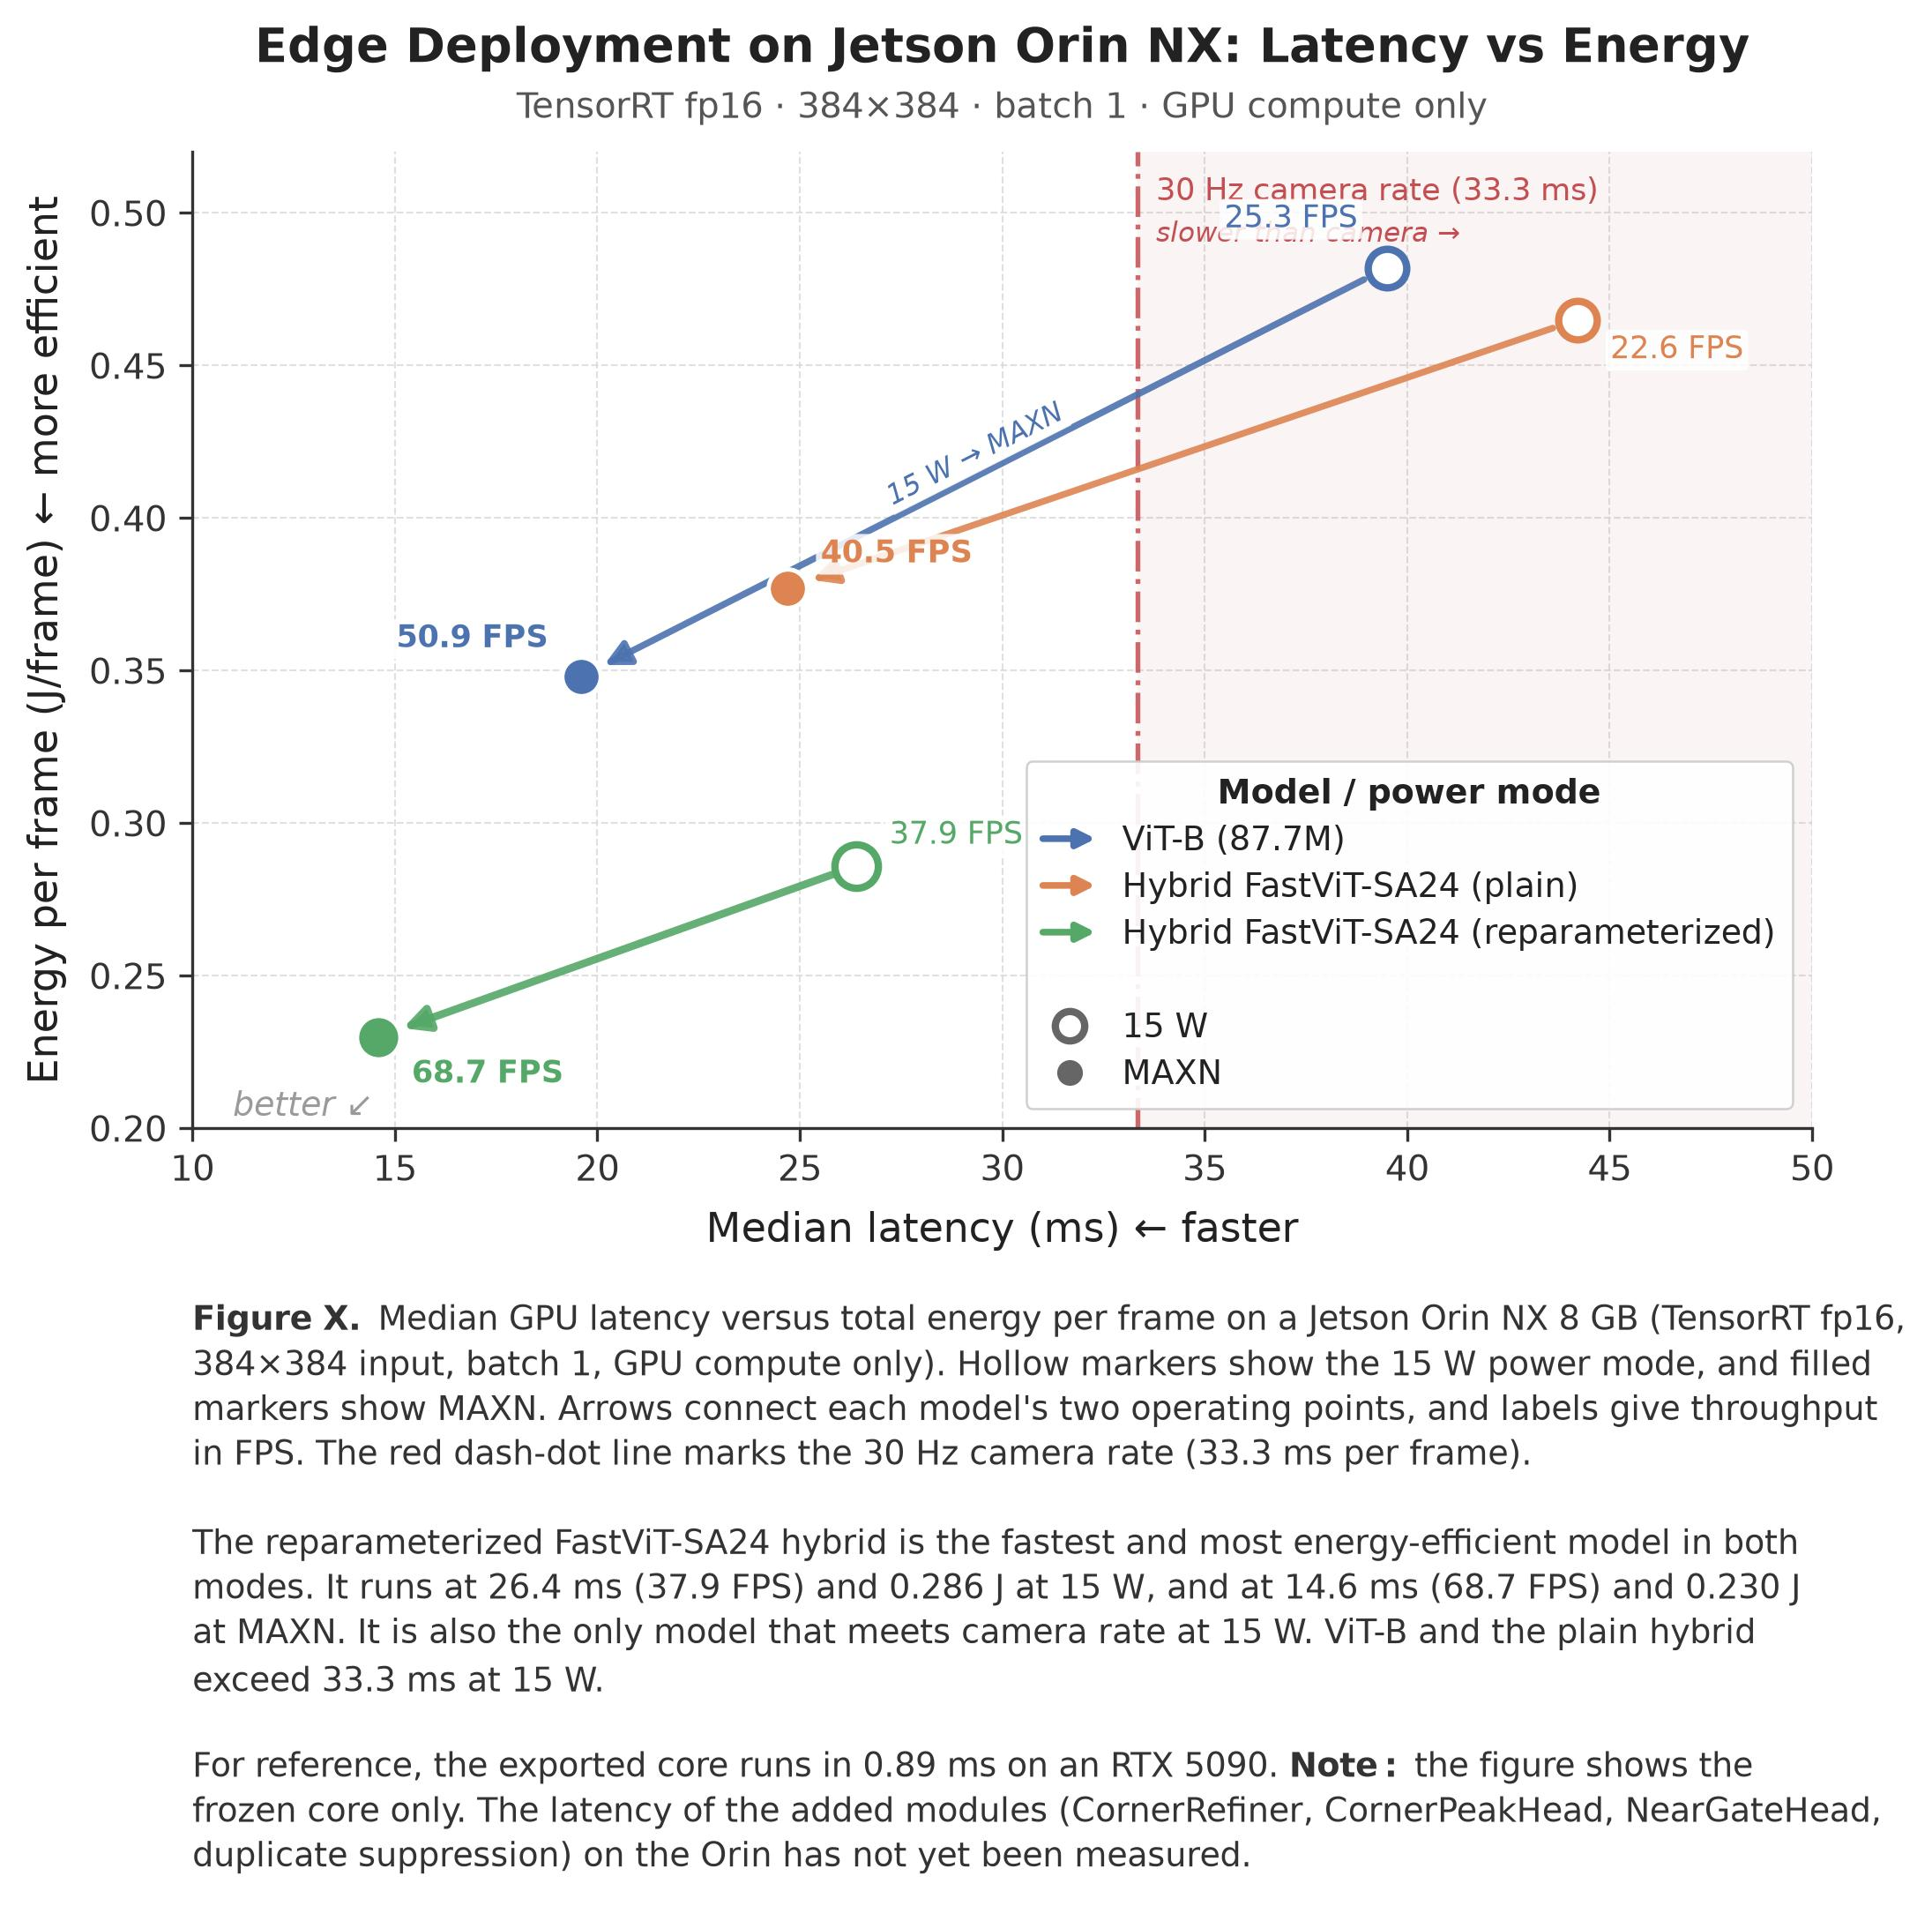
\includegraphics[width=\linewidth]{figures/fig_edge_latency_energy_jetson_orin.jpg}
  \caption{Median GPU latency vs.\ total energy per frame on a Jetson Orin NX 8\,GB (TensorRT fp16, 384$\times$384, batch 1, GPU compute only). Hollow markers: 15\,W; filled markers: MAXN; arrows link each model's two operating points, labels give FPS. The dash-dot line marks the 30\,Hz camera rate (33.3\,ms). The reparameterized FastViT-SA24 hybrid is fastest and most energy-efficient in both modes and is the only model that keeps up with the camera at 15\,W. Timings cover the frozen core only.}
  \label{fig:edge}
\end{figure}

We measure the core on a Jetson Orin NX 8\,GB with TensorRT fp16 at 384$\times$384, batch 1, counting GPU compute only (\cref{tab:edge}, \cref{fig:edge}). Structural reparameterization is essential. The plain hybrid runs at 44.2\,ms in 15\,W mode, slower than a ViT-B with 87.7M parameters (39.5\,ms). Both are slower than the 30\,Hz camera at 15\,W. After reparameterization the hybrid runs at 26.4\,ms (37.9\,FPS) at 15\,W and 14.6\,ms (68.7\,FPS) at MAXN, using 0.286 and 0.230\,J per frame, the lowest energy of the three models in both modes. On an RTX 5090 desktop GPU the exported core runs at 0.89\,ms.

\paragraph{Budget for the full detector.}
These measurements cover the shared core, which the robot runs anyway for its general tasks. Against the 33.3\,ms camera period, the reparameterized core leaves 6.9\,ms of GPU headroom at 15\,W and 18.7\,ms at MAXN. The application-specific part consists of three heads operating on the already computed stride-8 features $F$, plus NMS and a size filter on at most a few boxes per frame. Structurally, this is head-level computation and not a second backbone pass over the image, as running a separate detector such as GateNet next to the core would require. The latency of the three heads and of the post-processing on the Orin has not yet been measured. The headroom above is the budget they must fit into, at 15\,W or with MAXN as the fallback.
%%%%%%%%% EXPERIMENTS %%%%%%%%%

\section{Conclusion}
\label{sec:conclusion}
%%%%%%%%% CONCLUSION %%%%%%%%%
We asked whether a released general multi-task perception model can serve a precision-critical application without being changed. The core stays frozen. Small application-trained heads read its stride-8 features, and two parameter-free filters adapt the output to the downstream estimator. In a third-party drone racing stack in Isaac Lab, swapping only the detector, this system completed 87.5\% of 128 flights on final-test seeds versus 82.0\% for the dedicated GateNet detector, which we interpret as parity. The general metrics of the core, from TuSimple lane IoU to segmentation mIoU on six benchmarks and real-gate corner accuracy, are unchanged with and without the modules. In this loop, in-loop pixel precision and duplicate-free outputs explained closed-loop success better than offline crop metrics, and attempts to retrain the core gave no closed-loop gain.

\paragraph{Limitations.}
All closed-loop results are in simulation; we have no real-flight results. We study one application and compare against one dedicated baseline. The advantage over GateNet is consistent across two independent final tests but not significant at $p<0.05$ (sign test $p\approx0.14$), so we claim parity, not superiority. Our estimator errors for far gates (8+\,m) are worse than GateNet's. The latency of the modules on the Jetson Orin NX has not yet been measured. The min-size sweep compares slightly different seed subsets. Precision is ultimately bounded by what the frozen features encode, and each added module adds head-level compute.

\paragraph{Broader impact.}
Perception for agile autonomous drones has dual-use potential. Our study is confined to simulated racing, and the design principle, preserving validated capabilities when extending a model, is primarily a safety and maintenance benefit.

\paragraph{Future work.}
The frozen-core principle suggests a self-expanding system. The vehicle would detect distribution shift onboard and generate targeted synthetic data for the failure mode, from 3D Gaussian Splatting reconstructions, simulation and LLM/VLM-driven scenario generation. It would then train a new module, verify it in the closed loop, and plug it in. Immediate next steps are real-flight validation, more final-test flights to resolve the statistical question, a size- or distance-aware detection filter for far gates, and onboard timing of the modules.
%%%%%%%%% CONCLUSION %%%%%%%%%

{
    \small
    \bibliographystyle{ieeenat_fullname}
    \bibliography{references}
}

%%%%%%%%% Appendix %%%%%%%%%
\clearpage
\appendix
\section{Full closed-loop log and seed protocol}
\label{sec:app_log}
\paragraph{Seed ranges, roles and flight counts.}
Every seed is flown by four drones, so a range of 8 seeds corresponds to 32 flights and a range of 16 seeds to 64 flights per arm. \emph{Validation seeds} were 31--38 and 41--56 (64 flights); the min8/min20 sweep used the subset 41--48 (32 flights). Settings such as the duplicate-suppression IoU and the min-size threshold were chosen on these seeds. \emph{Development-check seeds} were 71--78 (step A, 32 flights), 91--98 (step D, 32 flights), 101--116 (step D, 64 flights) and 121--136 (step E, 64 flights). Each range was evaluated once, after the corresponding step, and never reused. Their outcomes and in-loop diagnostics influenced which direction we pursued next, so we do not treat them as held out. \emph{Final-test seeds} 141--156 and 161--176 (64 flights per arm each, 128 in total) were not examined in any form before the final configuration, including min14, was frozen. The step results are listed in \cref{tab:path} and visualized in \cref{fig:path}.

\paragraph{Loop noise.}
A flight's outcome depends on the random track, the quadrotor parameters and the interaction of perception errors with the policy. Repeated evaluations with 32 flights varied by about $\pm$10--15 success points. For reference, the binomial standard error at $p\approx0.8$ and $n=32$ is about 7 points, and track-level correlation among the four drones of one seed increases the effective variance further. This motivates (i) separating validation and test seeds, (ii) using 64 flights per arm per final test, and (iii) reporting a seed-level sign test instead of relying on raw percentage differences. The per-distance estimator errors for both final tests are given in \cref{tab:ekf}.

\section{Negative results and general-metric details}
\label{sec:app_neg}
\paragraph{Core retraining attempts.}
We tried to raise corner precision inside the core in four ways: (i) retraining or fine-tuning on simulator renders of the racing environment, (ii) increasing the corner loss weight to 10, 40 and 100, (iii) a stride-2 dense corner head instead of stride 4, and (iv) model soups of variants. None of them yielded a closed-loop gain beyond loop noise in our checks. The degradation of general metrics grew with the corner loss weight. Each attempt also produces a new core whose general metrics must be re-validated across all benchmarks, which the frozen-core design avoids.

\paragraph{Failed output-interface variants.}
Three variants targeted the output interface rather than precision: re-ordering corners to an identity order, geometric sorting of near-gate detections, and adding small near-gate detections without deduplication. All of them reached only 15.6\% success. The offline duplicate rate (0.317 per frame with small adds, versus 0.054 for val\_H and 0.018 for GateNet) was the only offline quantity that signalled the problem.

\paragraph{Per-seed general metrics.}
\Cref{tab:seeds} reports the general metrics that varied across three 16-epoch training seeds of the core. Release v4 corresponds to the values in \cref{tab:general}.

\begin{table}[h]
  \centering
  \small
  \begin{tabular}{@{}lccc@{}}
    \toprule
    Metric & Seed 1 & Seed 2 & Seed 3 \\
    \midrule
    Red, within 10\,px & 0.939 & 0.958 & 0.958 \\
    TuSimple lane IoU & 0.803 & 0.803 & 0.804 \\
    Aeroscapes drone IoU & 0.675 & 0.614 & 0.539 \\
    \bottomrule
  \end{tabular}
  \caption{Variation across three 16-epoch training seeds of the core.}
  \label{tab:seeds}
\end{table}

\paragraph{Edge measurement settings.}
All Orin measurements use a Jetson Orin NX 8\,GB, TensorRT fp16 engines, 384$\times$384 input, batch 1, and report median GPU compute latency. Energy per frame is the total energy over the inference interval divided by the number of frames, in the 15\,W and MAXN power modes. Moving from 15\,W to MAXN roughly halves latency for all models (\eg 26.4$\to$14.6\,ms for the reparameterized hybrid) and also reduces energy per frame (0.286$\to$0.230\,J), since the shorter run time outweighs the higher power draw.
%%%%%%%%% Appendix %%%%%%%%%

\end{document}